\chapter{Temporal Models of Student Behavior}\label{chap:hmm} 

In the previous chapter we presented a flat discriminative model to be able to predict \sti. In this chapter we present a methodology to model a student's data temporally. We posit that while taking a course a student has a latent state that represents a summary of his \textit{engagement} and \textit{interest} in the course during a particular week $i$. The \feat that we evaluated for the student for a week $i$ represent a draw from a multivariate distribution pertaining to that state. We posit that a student transitions from one state to another state during the course as the course transitions from one week to another. Using the data from multiple students our goal is to identify how many unique states there are, how students transition from state $i$ to state $j$ and what multivariate distribution of the \feat does each state represent? 

One way to achieve this is to cluster all students weekly data which is $15 \times N$ number of data points. Next, extract every student's cluster label on a weekly basis. We can then learn the transitions between the cluster labels across all students. An alternative approach presented in this chapter uses Hidden Markov Models (HMM) to jointly identify the multivariate distributions that each state represents and the transition probabilities between states.  

\section{Hidden markov models for modeling student behavior}
Hidden markov models, or HMMs, are a powerful and highly used class of \textit{generative} models. HMMs are usually built to model time series data, such as stock prices. They are a type of probabilistic graphical models in which the modeled entity is assumed to transition from one latent state to another as discrete time steps progress.  However, this state is not directly observable, and thus is `hidden.'  HMMs suppose that although the hidden state is not directly observable, the state relates to variables that are observable probabilistically. More specifically, each hidden state corresponds to a multivariate distribution for the observed variables from which they are most likely sampled from given the hidden state. The most basic HMM has only one observed variable (per time step), but the models we create contain 28 observed variables, one per feature\footnote{Most software libraries only support one observed variable. This is because using multiple observed variables is computationally complex}. Figure \ref{fig:hmm} shows the graph structure of a typical HMM. In the figure, Z (shaded node) represents a hidden node. The graphical form as shown in the Figure~\ref{fig:hmm} can be written as a joint distribution given by: 

\begin{equation}
p(z_{1:T},\bar{x}_{1:T})=p(z_1)\prod_{t=2}^T p(z_t|z_{t-1}) \prod_{t=2}^T p(\bar{x}_t|z_t)
\end{equation}
In the most common case, independence is assumed among the observed variables given the hidden variable, making the joint distribution:
\begin{equation}
p(z_{1:T},\bar{x}_{1:T})=p(z_1)\prod_{t=2}^T p(z_t|z_{t-1}) \prod_{t=2}^T \{ \prod_{i=1}^m p({x^i}_t|z_t)\}
\end{equation}

The observed variables can be either continuous, or discrete. In the continuous case, the distribution for observed variables is typically assumed to be independent univariate Gaussian. In the discrete case, a multinomial distribution is used to represent the joint distribution between the hidden variable and the observed variable.  Note that, when using multinomial distribution, observed values are no longer ordinal, but are nominal, i.e., A is not greater or less than B, rather is simply not B. To use this model when the variables are continuous the variables are binned using a methodology that preserves the entropy of the univariate distribution for that variable (presented in section \ref{section:binning}).

Let us assume that the hidden variable takes one of the $k$ values $1 \dots K$ and each observed variable has $1 \dots P$ discrete values. The model is parametrically defined by a $K$-by-$K$ transition matrix and $m$,  $K$-by-$P$ emission matrices, one for each of the observed variable given the hidden variable and a 1-by-K probability vector for the initial state $p(z_1)$. 

The entry $i,j$ in the transition matrix shown below represents the probability $p(z_t=i |z_{t-1}=j)$ and is given by: 
\begin{equation}
A_{i,j} =
 \begin{pmatrix}
  a_{1,1} & a_{1,2} & \cdots & a_{1,k} \\
  a_{2,1} & a_{2,2} & \cdots & a_{2,k} \\
  \vdots  & \vdots  & \ddots & \vdots  \\
  a_{k,1} & a_{k,2} & \cdots & a_{k,k}
 \end{pmatrix}
\end{equation}

and the emission matrix for $p^{th}$ observed variable is given by:

\begin{equation}
E_{i,j} =
 \begin{pmatrix}
  e_{1,1} & e_{1,2} & \cdots & e_{1,p} \\
  e_{2,1} & e_{2,2} & \cdots & e_{2,k} \\
  \vdots  & \vdots  & \ddots & \vdots  \\
  e_{k,1} & e_{k,2} & \cdots & e_{k,p}
 \end{pmatrix}
\end{equation}


The entry $i,j$ in the emission matrix for variable $m$ represents $p(x_t^m=i | z_t=j)$. The objective of training an HMM is to find the optimal \textit{transition} and \textit{emission} probabilities given the graphical structure. 
\begin{figure}[ht!]
  \caption{A typical hidden markov model structure. Top figure shows a common hidden markov model with only one variable. The bottom figure represents our case where we have multiple observed variables per time slice.}\label{fig:hmm}
  \centering
    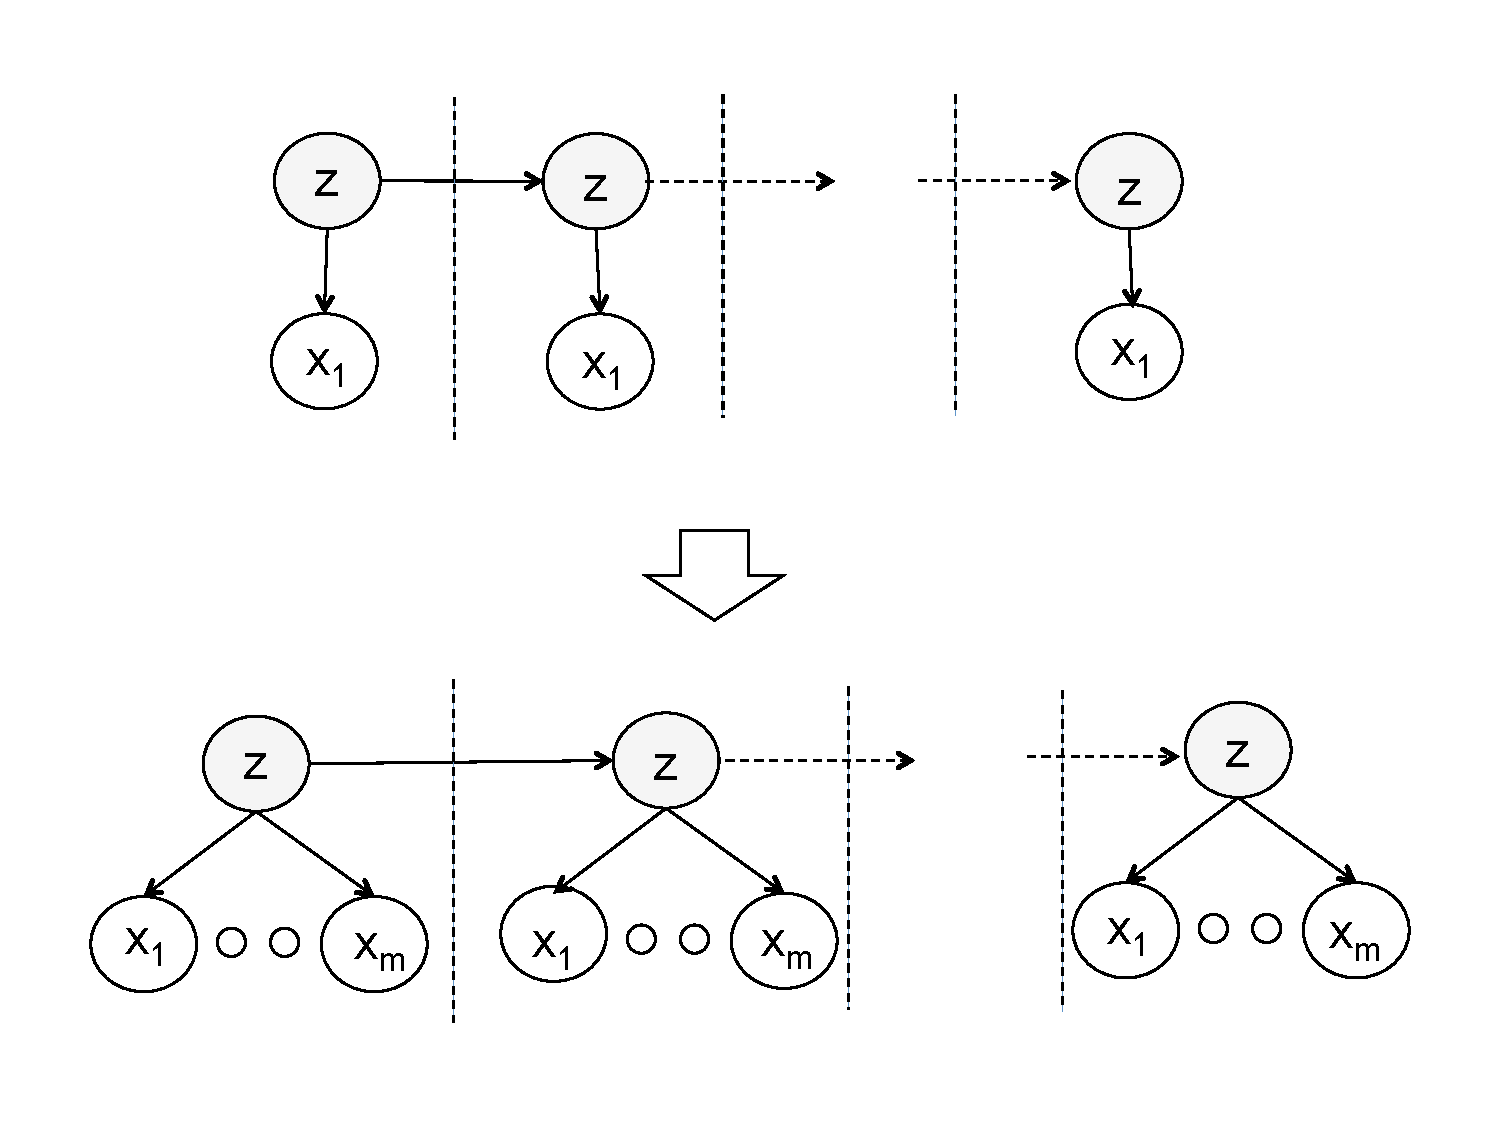
\includegraphics[width=1.0\textwidth]{figures/one-vs-multi}
\end{figure}

\subsection{Learning the probabilities of an HMM}
A hidden markov model is typically constructed using the Baum-Welch algorithm. Firstly, the initial states, transition matrices and emissions matrices are assigned (usually randomly). In each iteration of Baum-Welch, a forward-backwards inference algorithm is used to estimate the $p(z_t|\bar{x})$ for all $t$ and for all sequences given the parameters. Subsequent to this estimation, the 
 the emissions and transition matrices are updated.  As the parameters are updated, a log-likelihood score is evaluated to measure how well the model fits the data. In each iteration, the likelihood improves, and will begin to converge on either a local or global maximum.The algorithm terminates after the difference between log-likelihood of two consecutive iterations falls below a threshold (implying convergence), or a maximum number of iterations is reached. Through training, the model learns both the distributions of observed variables for each state, and the probabilities of transitioning from one state to another.

Figures \ref{fig:hmm_training} demonstrates how the observed variables are used as evidence in order to train the HMM.


\begin{figure}[ht!]
  \caption{This figure shows how the student-week-matrix which has features that represent the behavior of a student during a week is provided as evidence to the hidden markov model training.}\label{fig:hmm_training}
  \centering
    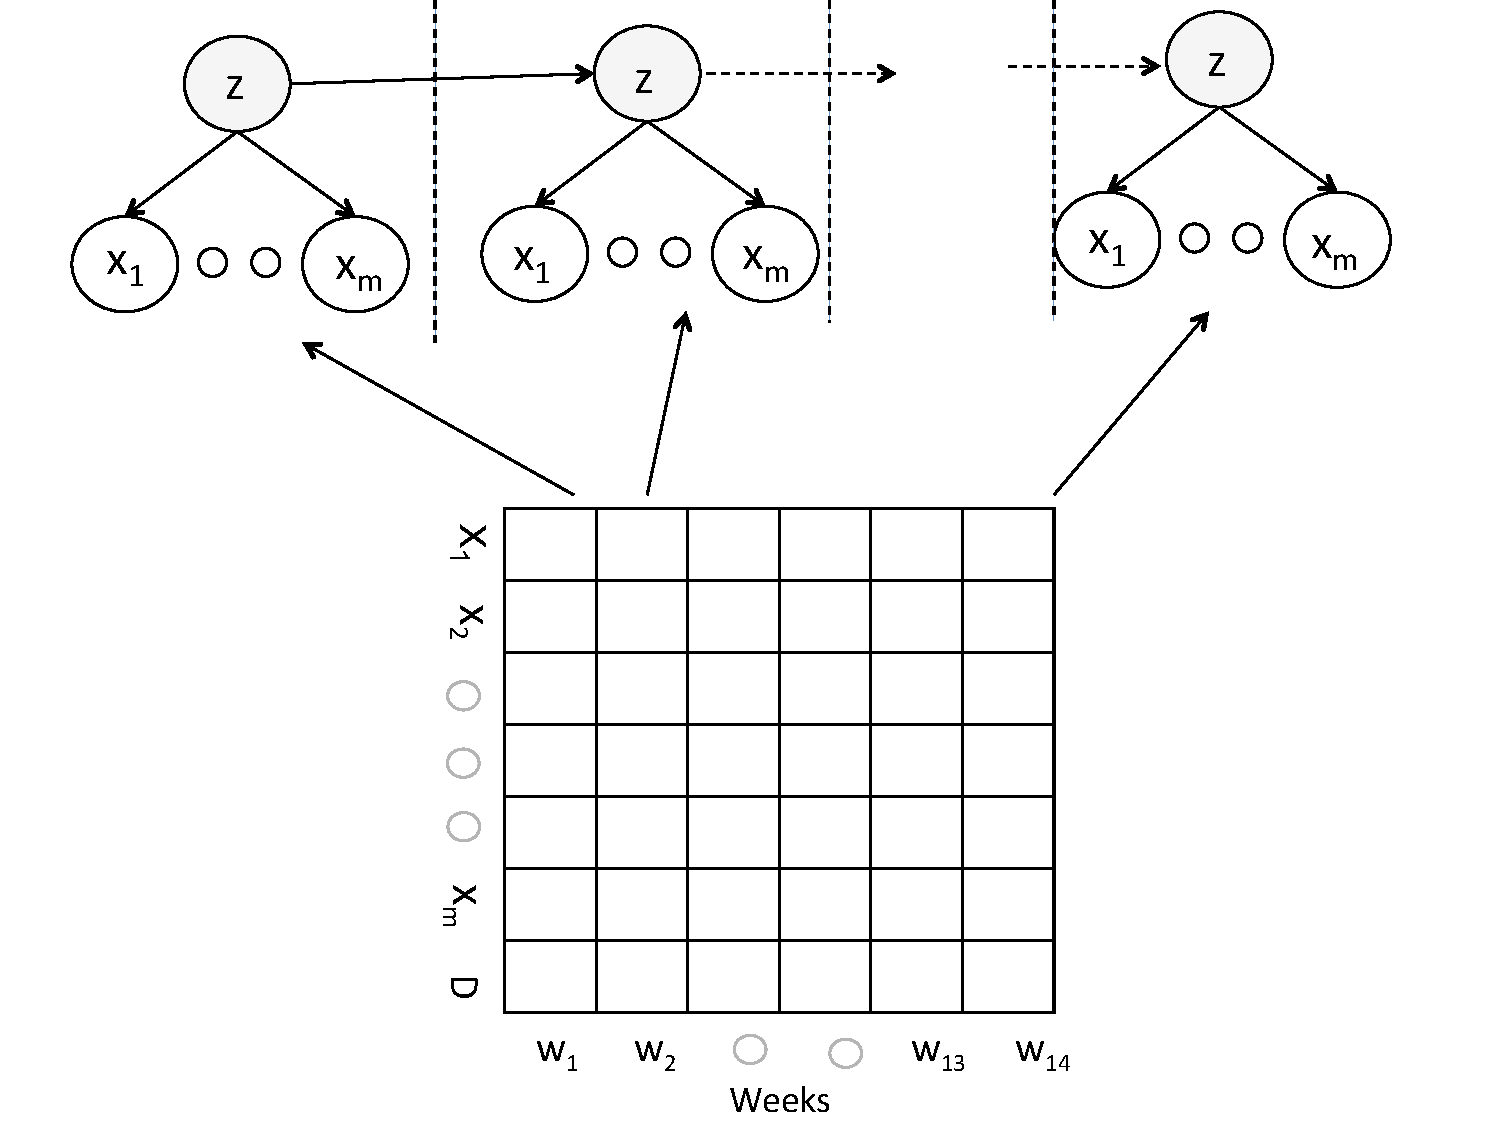
\includegraphics[width=0.7\textwidth]{figures/week_matrix_to_hmm}
\end{figure}

\subsection{Inference}
Once the HMM is built, we can utilize it to predict a future value of an observed variable. In our case, we can predict the \sti variable for a future week. Figure \ref{fig:hmm_predict} shows this use of an HMM as a prediction engine. An alternative inference goal is to find the probabilities for each hidden state at a given future timestep. Inference is performed using the forward-backwards algorithm.

\begin{figure}[ht!]
  \caption{This figure shows how the HMM is used to predict value for an observed variable in a future time slice. In this specific example evidence is provided to the model through week 2 and a prediction is sought for the 14th week }\label{fig:hmm_predict}
  \centering
    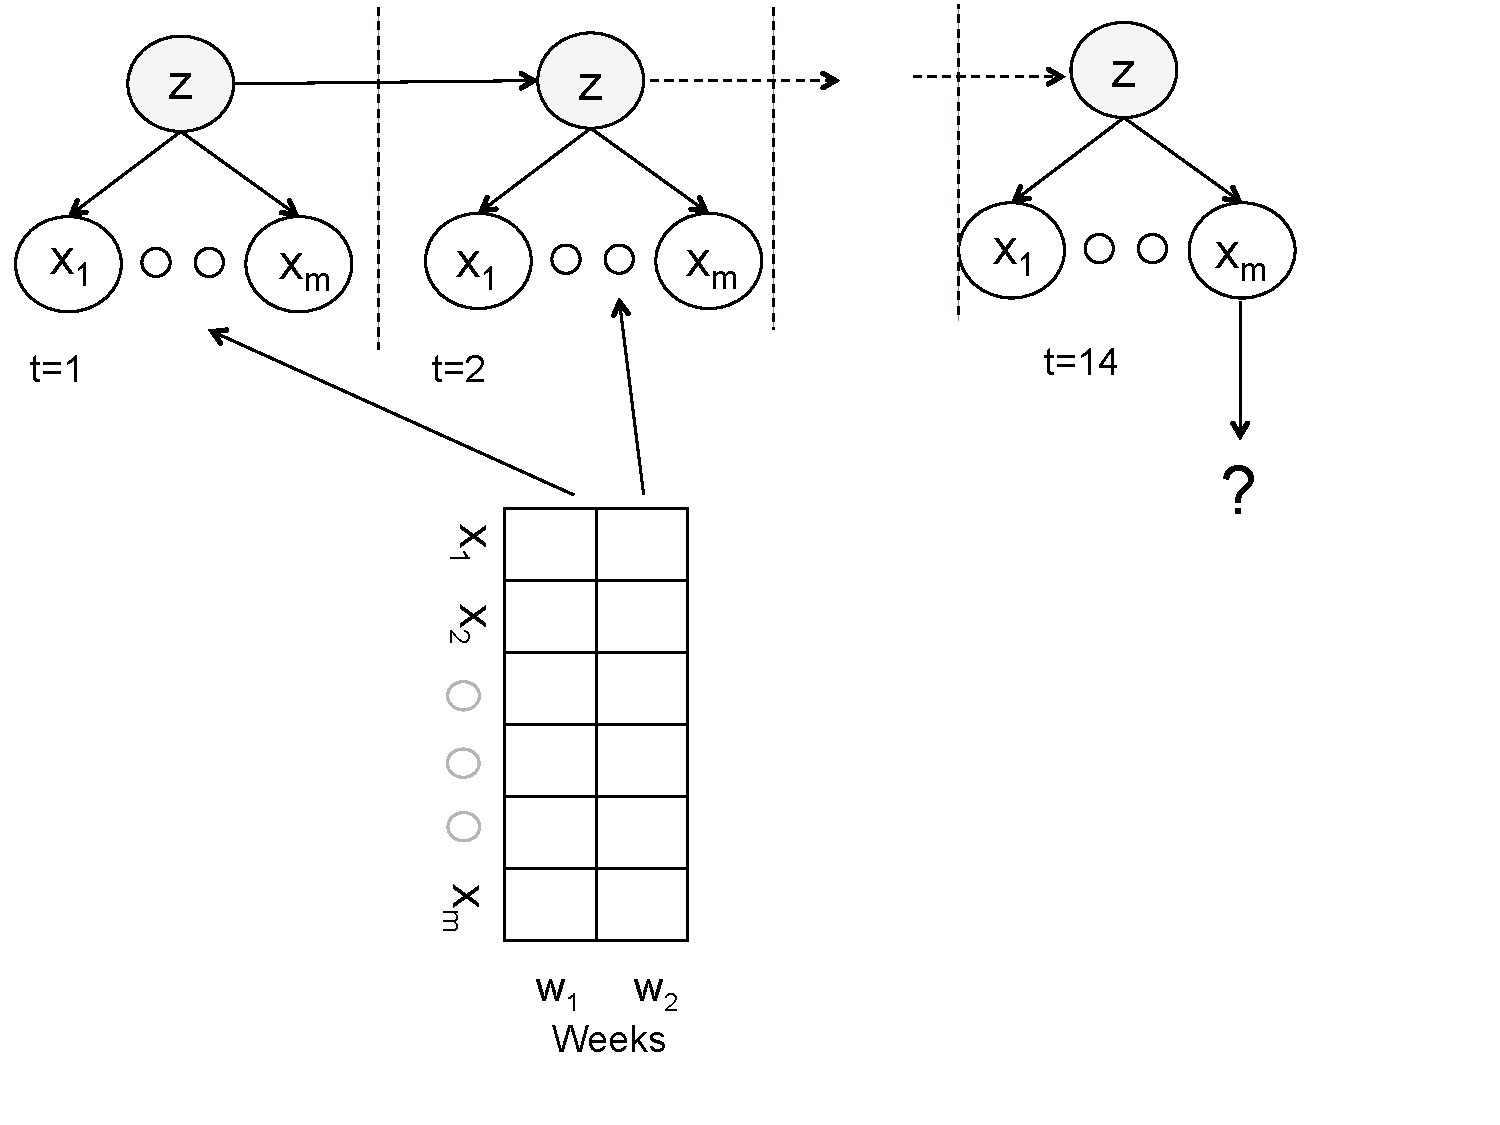
\includegraphics[width=0.7\textwidth]{figures/hmm-as-predict}
\end{figure}

\subsection{Advantages and disadvantages of HMMs} 
\begin{itemize}
\item Hidden markov models are designed for time sequenced data. They allow for repeating features across time sequences. 
\item HMMs hidden state provide some intuitive notion of clustering types of students by way of the hidden state. For example, if a model with a hidden support of 4 delivers fantastic predictive power, we could surmise that there are really 4 modes an entity can be in. Indeed, the emission probabilities of the hidden states might provide insights about what the modes may represent. In the stopout prediction problem, for example, the modes might represent different levels of engagement in the course, and represent the true state of a student in a given timestep. However, apart from such a scenario, HMMs often become a black box predictive model. For example, there is no notion of feature weights. 
\item HMMs require a lot of computing power to train, and the training time grows exponentially with the number of time sequences (this is offset through dynamic programming techniques, but is still slow). 
\item Hidden markov models assume independence between the observed variables given a hidden variable, which is often not the case (such as in our feature-set which uses derived features). Training a more complicated graph is possible, but much more computationally intensive.
\item The Baum-Welch algorithm can get stuck on local maxima of probabilities as it converges.
\end{itemize}

\section{Predicting stopout using HMMs}
We trained hidden markov models with the objective of predicting student persistence. We used the 28 (27 interpretive features + binary stopout feature) as described in chapter 3 as the observed variables of the hidden state. We applied inference to the trained models, asking the HMM to generate the probabilities of sampling the \sti value for a future timestep.

Each experiment used a given lead as a parameter. For example, for a lead of 1, we used features from week 1 to predict week 2, then features from 1 and 2 to predict week 3, etc. Note that this prediction problem is subtly different from that of the logistic regression. In logistic regression, we chose a lead and a lag, and predicted a single week's stopout value. Here, we choose a lead, and use every possible lag with that lead in order to predict every week up until the end of the course. However, as in logistic regression, we do not perform inference on weeks where the student is already known to have stopped out.

Hidden markov models require several parameter choices. Because the correct hidden support value is unknown in hidden markov models, we varied this parameter to find an optimal value. We used a range of supports from 3 to 29, with a step size of 2. We stopped at 29 for the sake of computing time. We used 100 iterations as the maximum number of Baum-Welch iterations along with a log-likelihood differential threshold of 0.0000001. Training stopped when one or the other was reached.

\subsection{Experimental setup}
To build a predictive HMM, we did the following on every lead, hidden support and cohort combination
\footnote{We first used a Matlab implementation of Dynamic Bayesian Networks in order to build HMMs. This toolbox was flexible enough to construct arbitrary graphical structures, including HMMs. However, this toolkit proved too slow to use, even at scale. We switched to a custom built implementation of hidden markov models. The code was written in C++ by two members in the ALFA group. It was orders of magnitude faster, but provided a much cruder interface to use. After a lot of testing, and benchmarking, we achieved as good of results as with the MATLAB implementation given a large dataset, and with much faster time. Consequently, we recommend any sizable machine learning/data science project to use C++}:

\begin{enumerate}
\item Performed 10 fold cross validation on the training set. In order to speed this process up, we ran each in parallel using python's Parallelization package.
\item Trained an HMM on the entire train dataset. To compensate for the fact that HMMs often get stuck on local maxima as they train, we trained 10 models for each experiment. We selected the best model to use based on the likelihood score of the Baum-Welch algorithm. We also performed this in parallel, as training can take significant amounts of time.
\item Performed inference on the test dataset by putting each data point through best model. Specifically, we asked the model for the probabilities of each stopout value for a given week. We compared the resulting probability of stopout versus the truth stopout label.
\item Evaluating the model using mean cross-validation ROC AUC and test set ROC AUC.
\end{enumerate}

\section{HMM results}
Our hidden markov models performed well at predicting stopout.  Overall, we saw a fairly sharp decline in accuracy as the lead increased, especially as compared with logistic regression. Similar to logistic regression, different cohorts achieved very different prediction accuracies as well.

\begin{figure}[ht!]
  \caption{Heatmap for the \neither cohort. PCA transformations of features used.}\label{fig:hmm_heatmap_no_collab_pca}
  \centering
    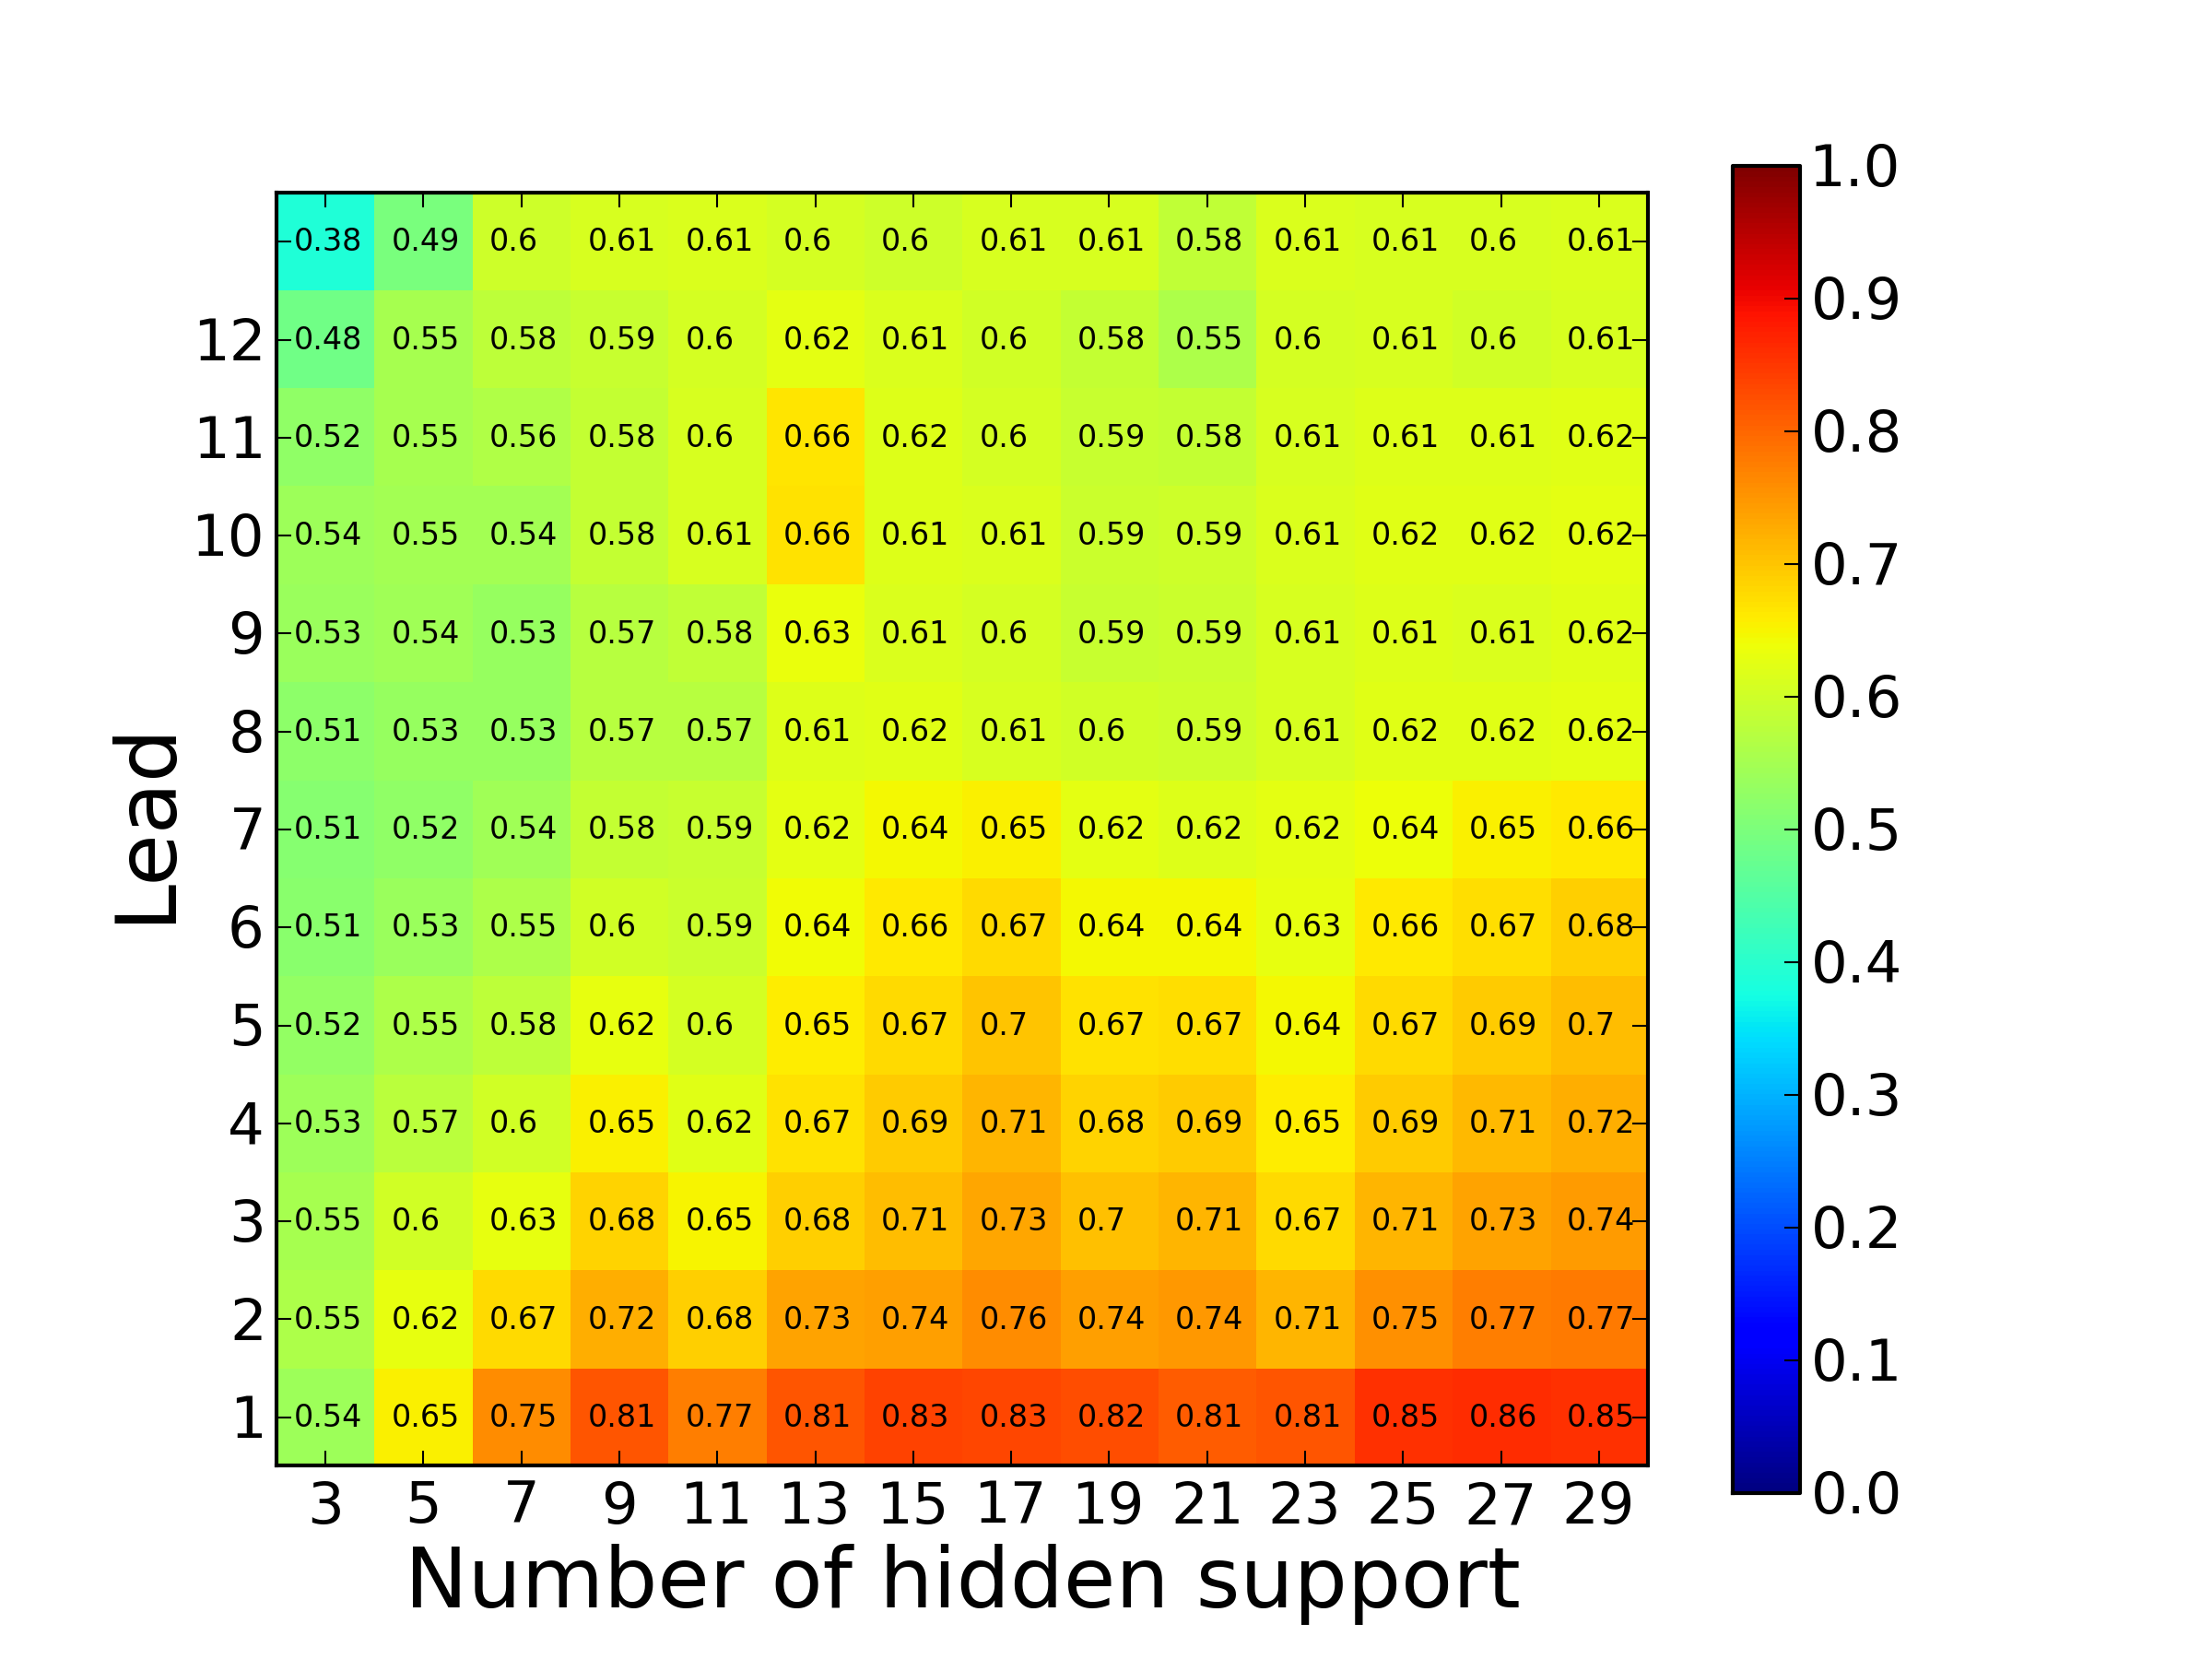
\includegraphics[width=1.0\textwidth]{figures/hmm/no_collab_pca.png}
\end{figure}

\begin{figure}[ht!]
  \caption{Heatmap for the \forum cohort. PCA transformations of features used.}\label{fig:hmm_heatmap_forum_only_pca}
  \centering
    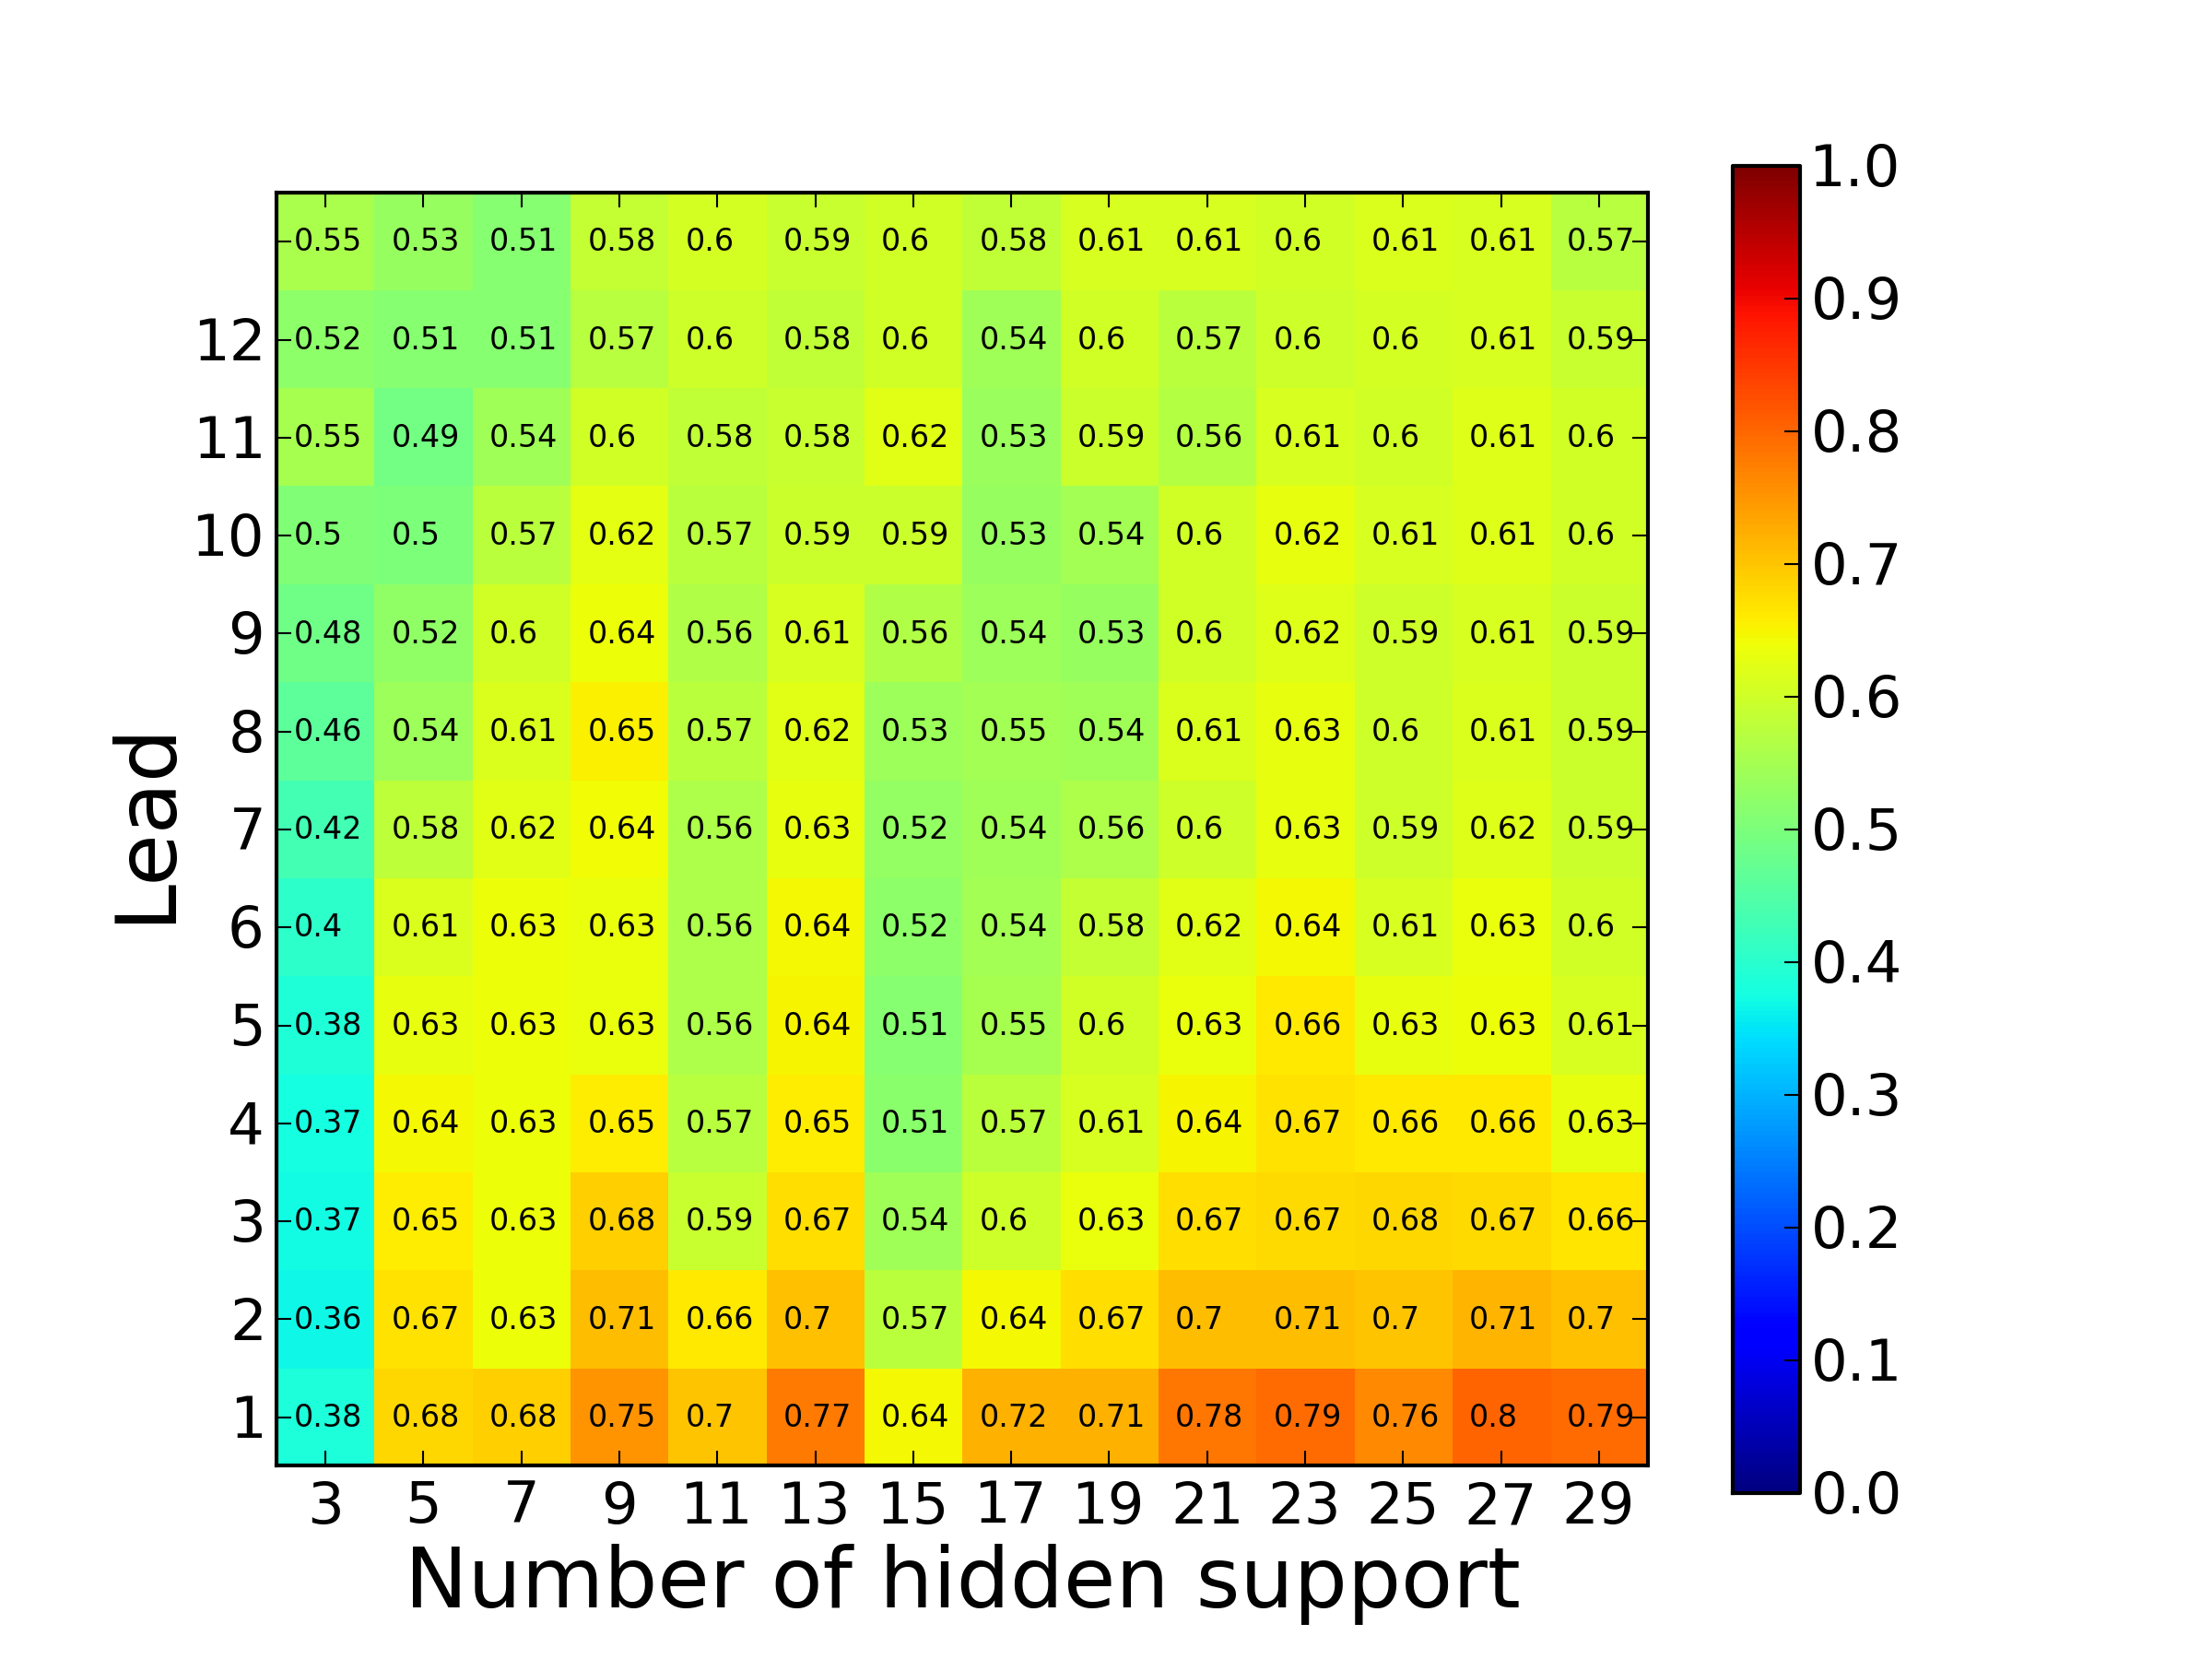
\includegraphics[width=1.0\textwidth]{figures/hmm/forum_only_pca.png}
\end{figure}

\begin{figure}[ht!]
  \caption{Heatmap for the \both cohort. PCA transformations of features used.}\label{fig:hmm_heatmap_forum_and_wiki_pca}
  \centering
    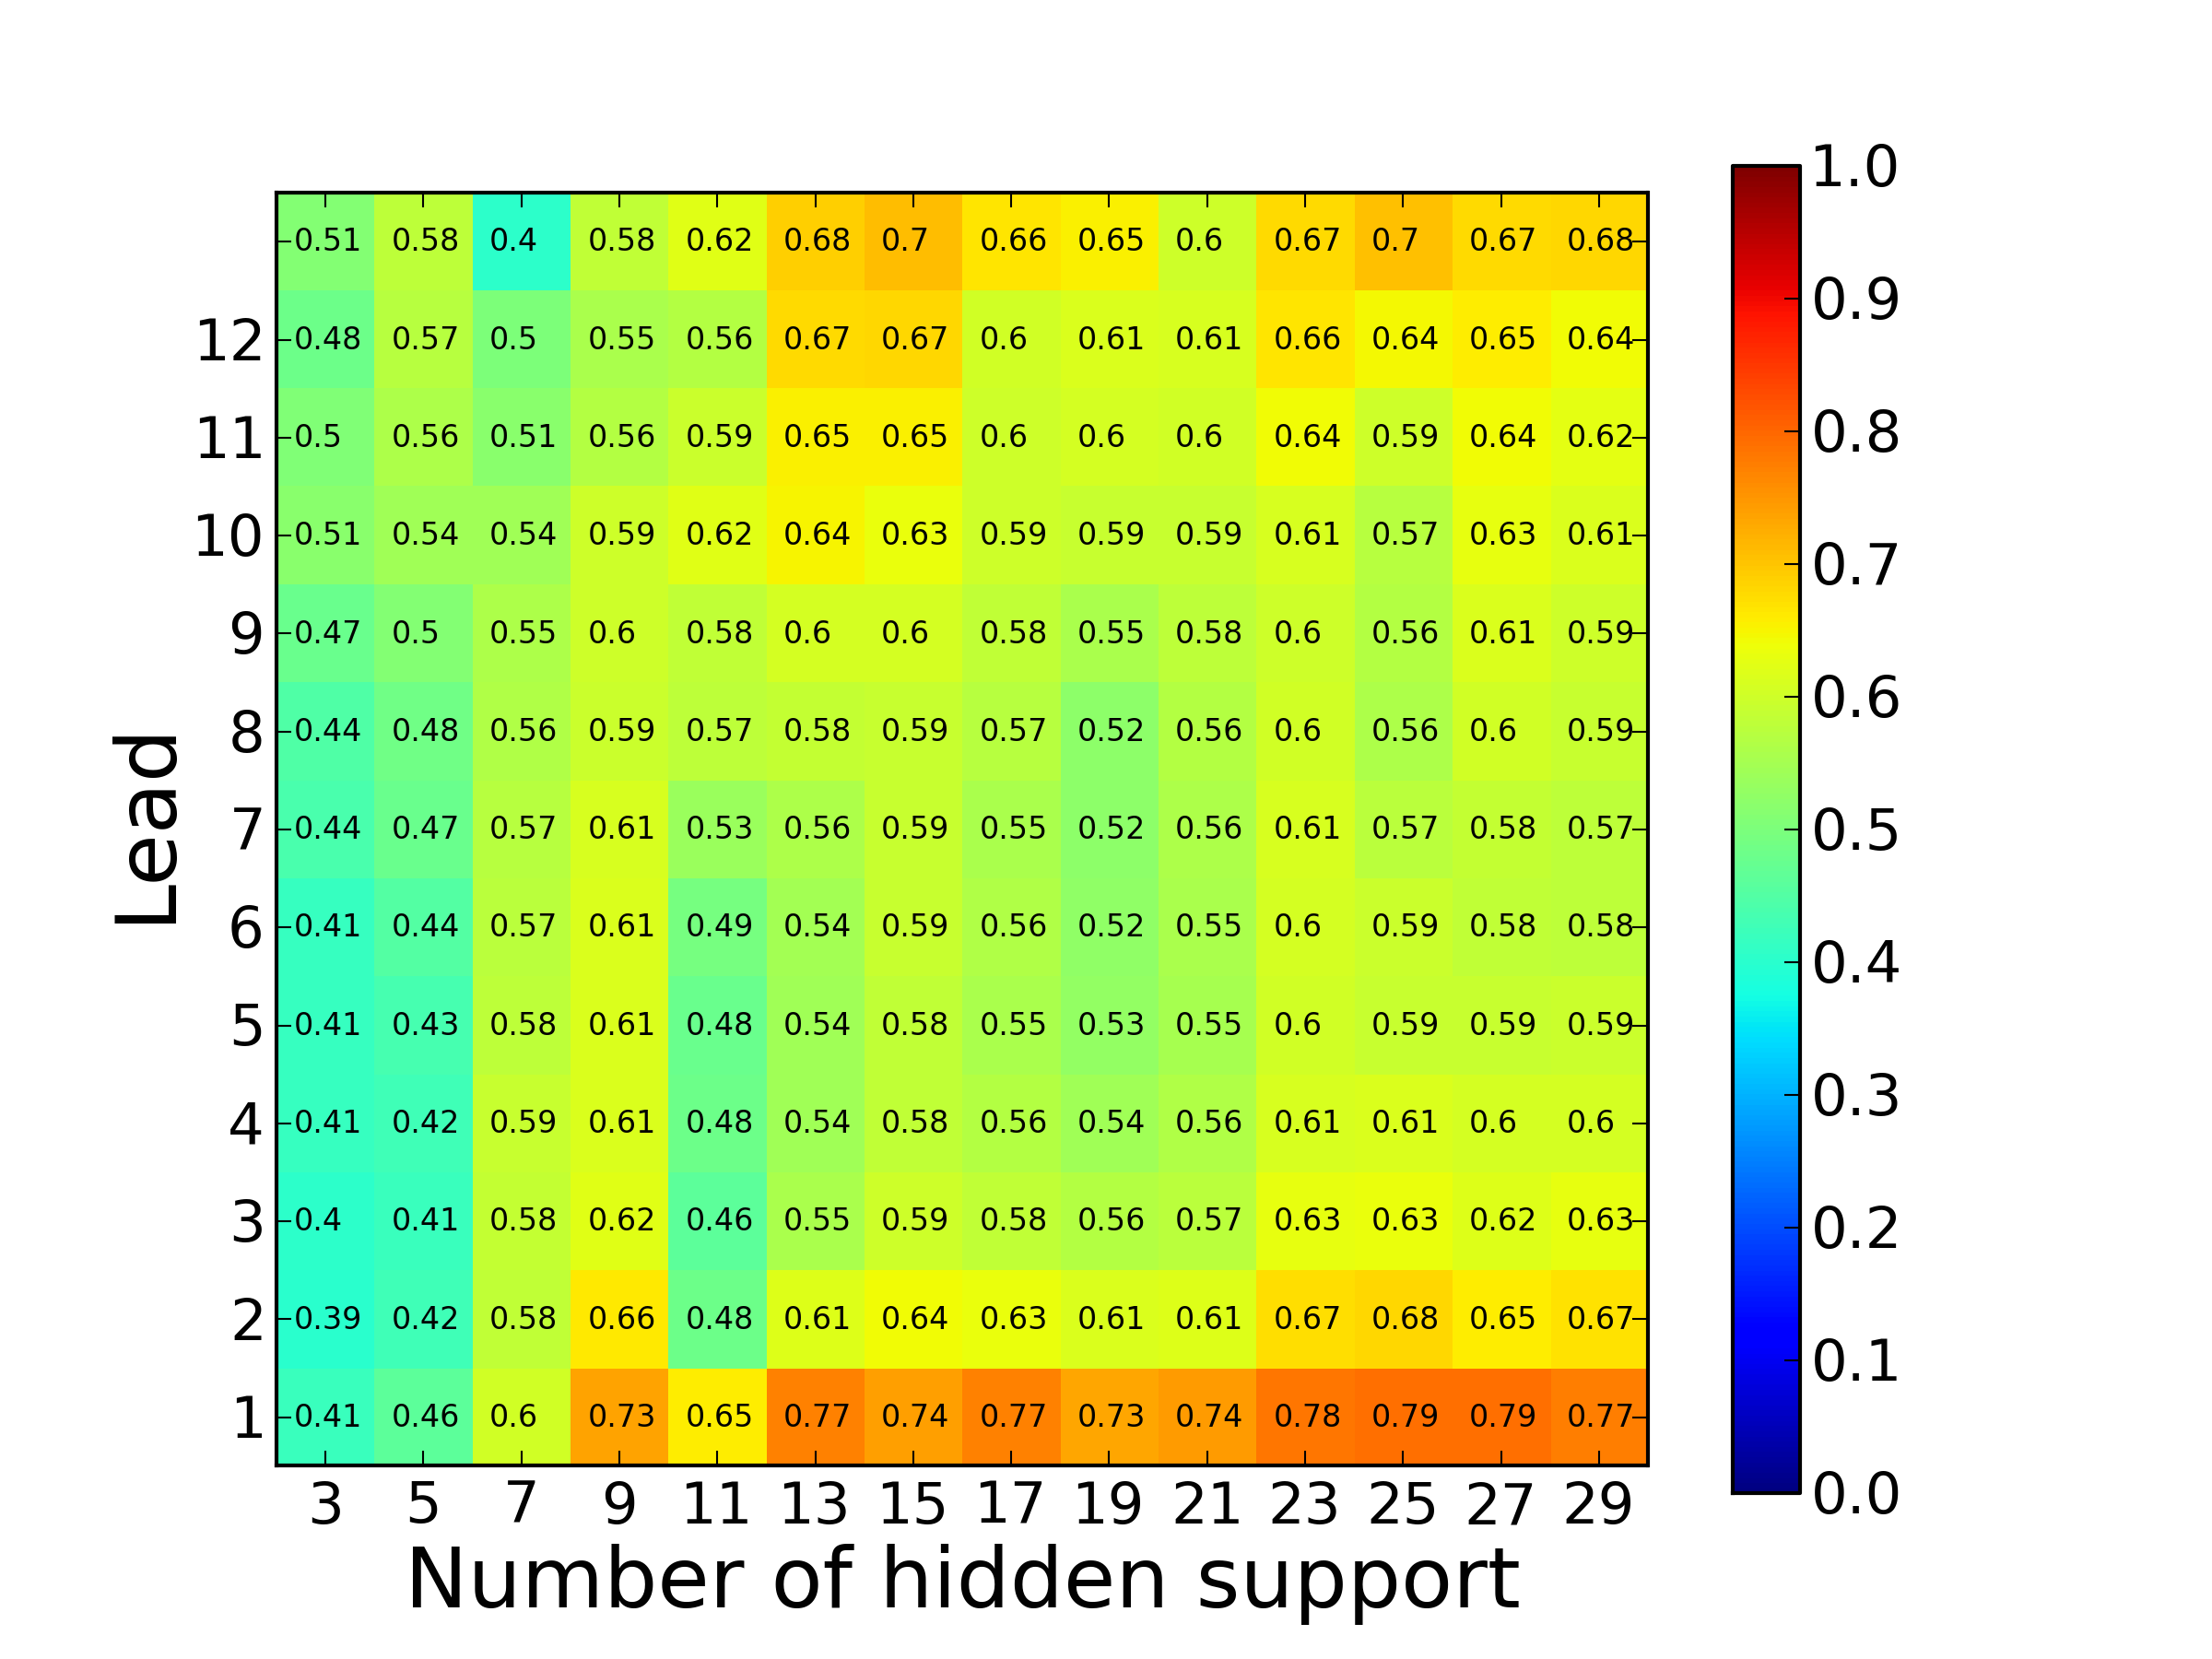
\includegraphics[width=1.0\textwidth]{figures/hmm/forum_and_wiki_pca.png}
\end{figure}

Figures \ref{fig:hmm_heatmap_no_collab_pca} to \ref{fig:hmm_heatmap_forum_and_wiki_pca} show HMM heatmaps for cohorts \neither, \forum and \both. These featuresets used PCA to reduce their dimensionality. We were unable to use PCA to reduce the \wiki cohort because it was too small. Each heatmap visualizes the ROC AUC for various leads as we vary K to create different models.

The PCA HMM models require a relatively larger K value in order to converge to a high AUC. For the \neither cohort, for example, we see that increasing K continually increases AUCs for all leads, up through a K of 29. This suggests that there are even more than 29 modes of students, and that we could attain even better results through a higher K value. The PCA HMMs show a large contrast between high leads and low leads. However, as compared with logistic regression, we see more consistent results cross the cohorts. For example, with a lead of one, the \neither, \forum and \both cohorts are within 0.08 of each other. In logistic regression, there is a difference in AUC of 0.2.

We suspect that the high difference in predictive accuracies between high leads and low leads is due to the fact that HMMs use a single transition matrix for all weeks. There is likely to be different probabilities of transferring hidden state between weeks 1 and 2 than between 12 and 13, for example, but the HMM posits only one set of probabilities. Furthermore, since there are more students in earlier weeks due to stopout, the transition matrix will have more examples from earlier weeks. Thus, it will be biased towards the earlier weeks, allowing for better prediction in the earlier weeks than in later weeks. 

\begin{figure}[ht!]
  \caption{Mean AUC as K increases for the \neither cohort. PCA transformations of features used.}\label{fig:hmm_support_over_time_no_collab_pca}
  \centering
    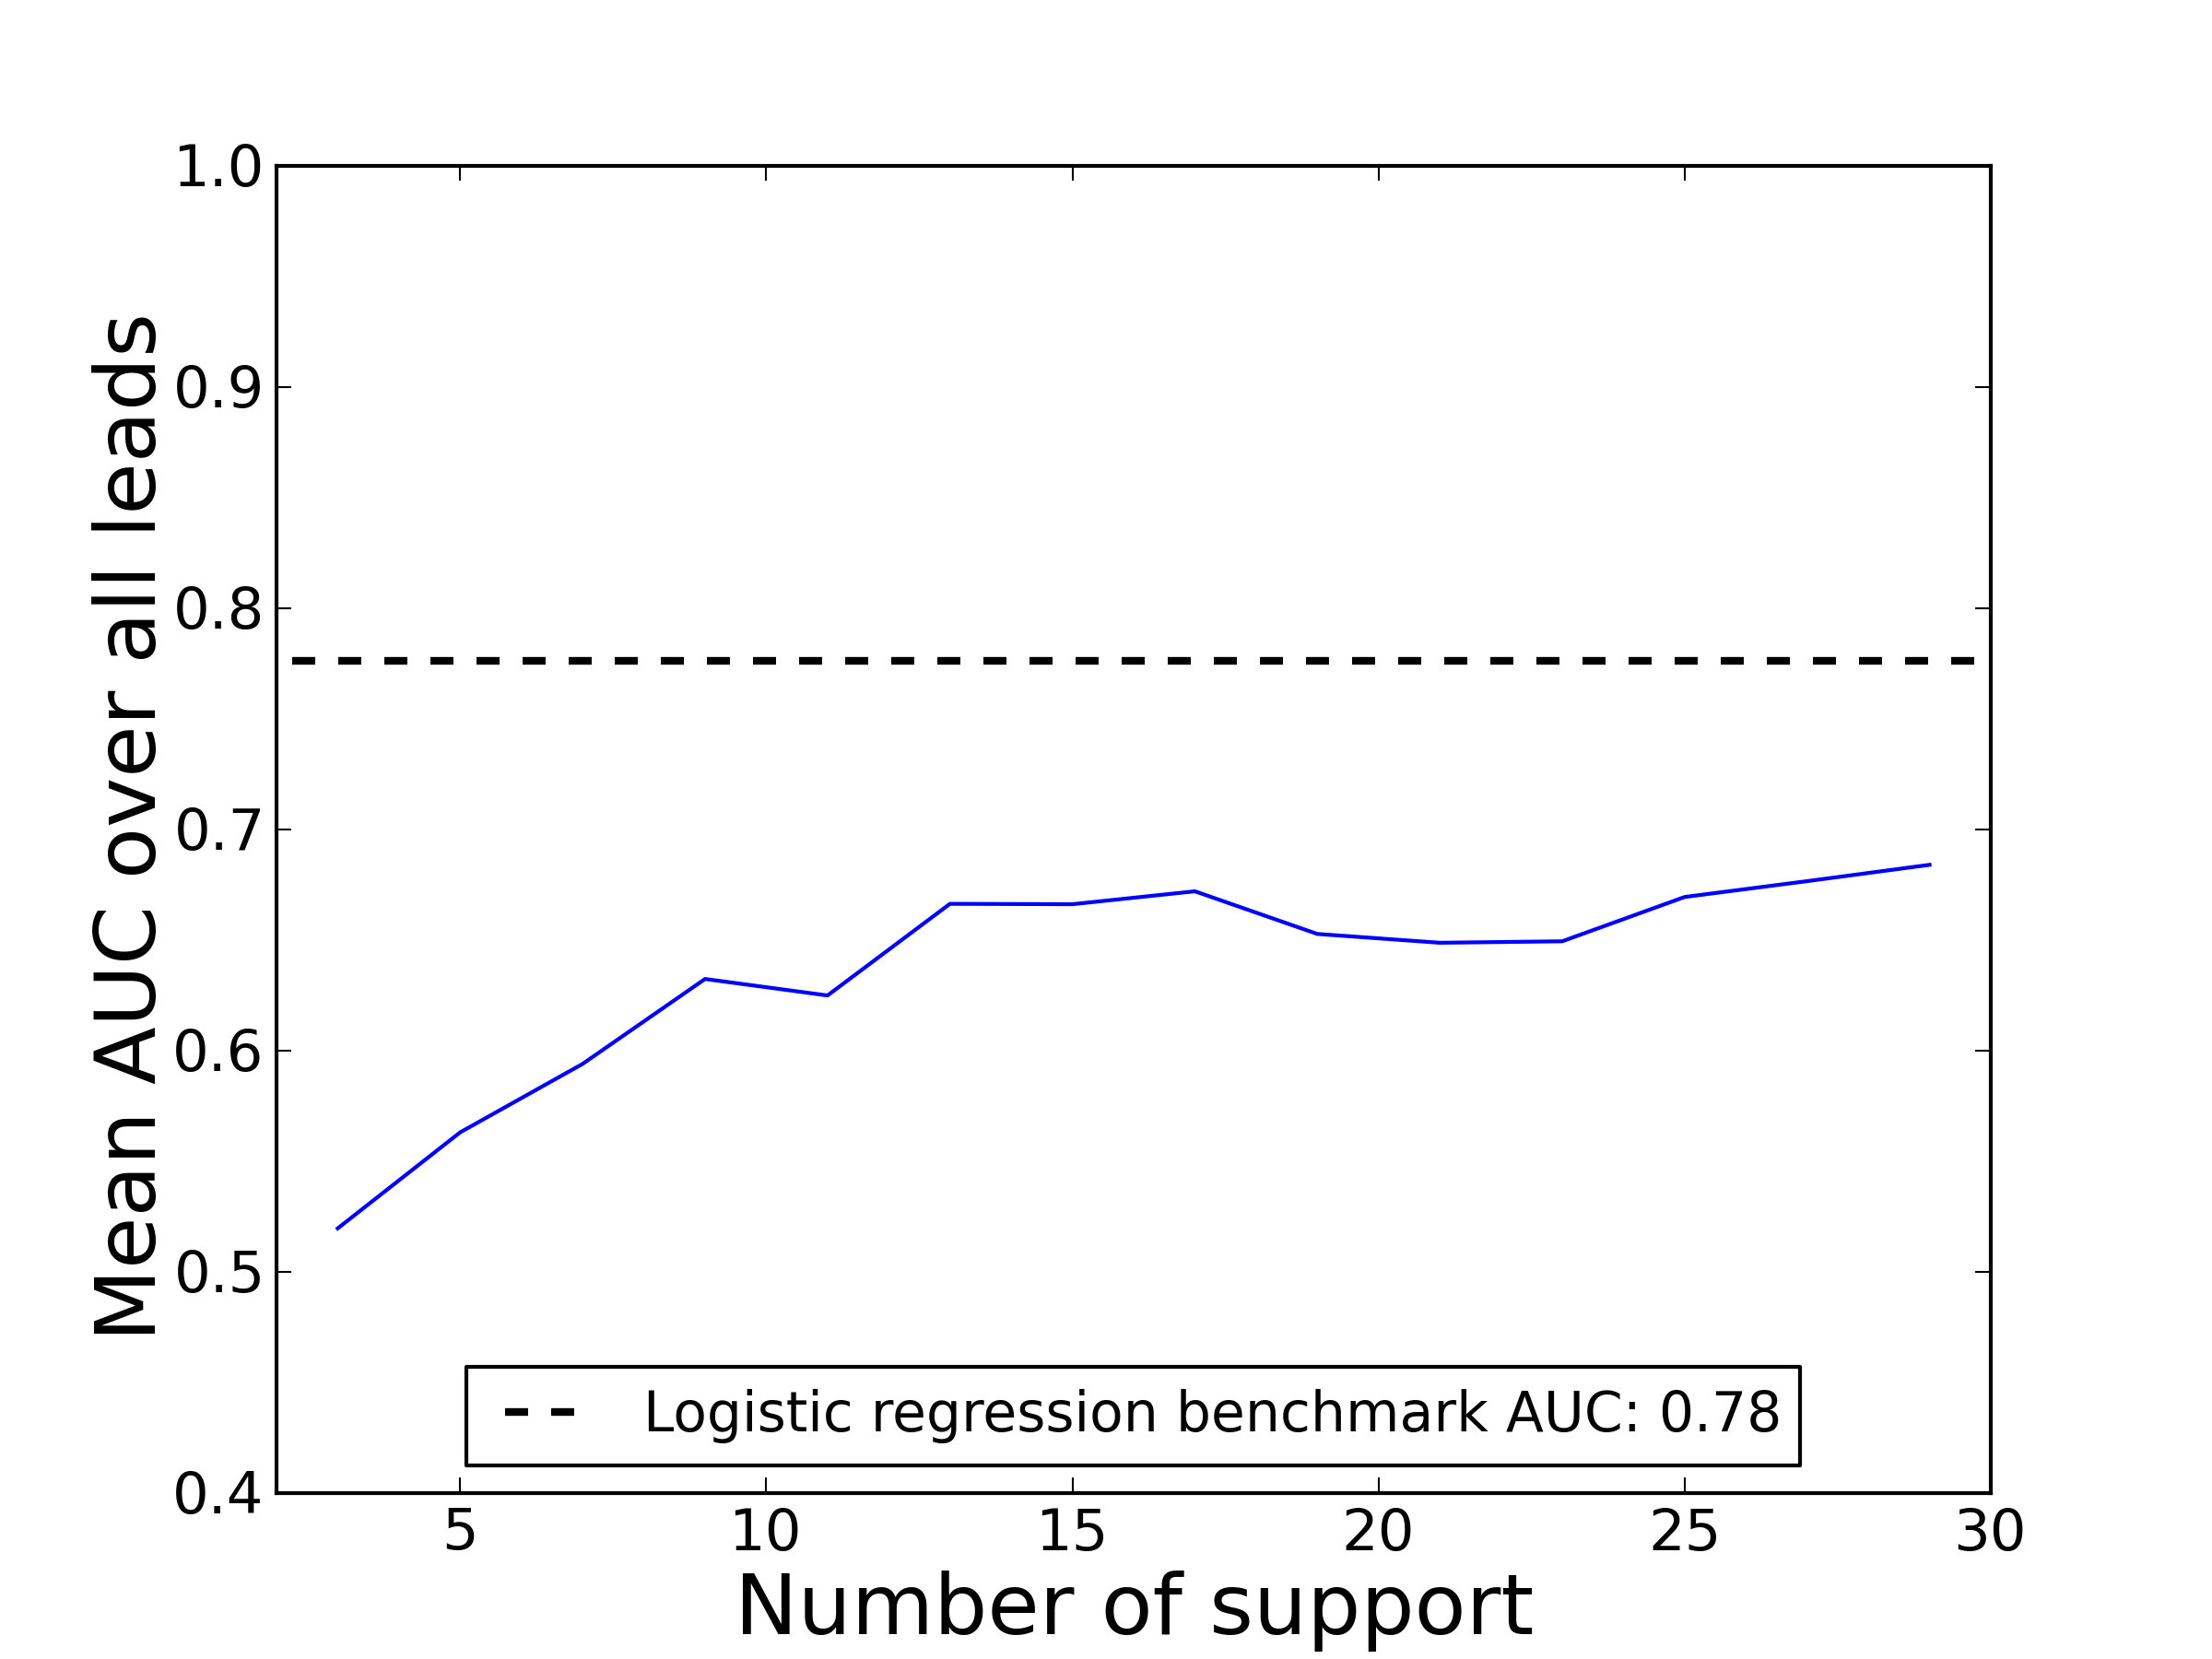
\includegraphics[width=0.8\textwidth]{figures/hmm/no_collab_pca_support_over_time.png}
\end{figure}

\begin{figure}[ht!]
  \caption{Mean AUC as K increases for the \forum cohort. PCA transformations of features used.}\label{fig:hmm_support_over_time_forum_only_pca}
  \centering
    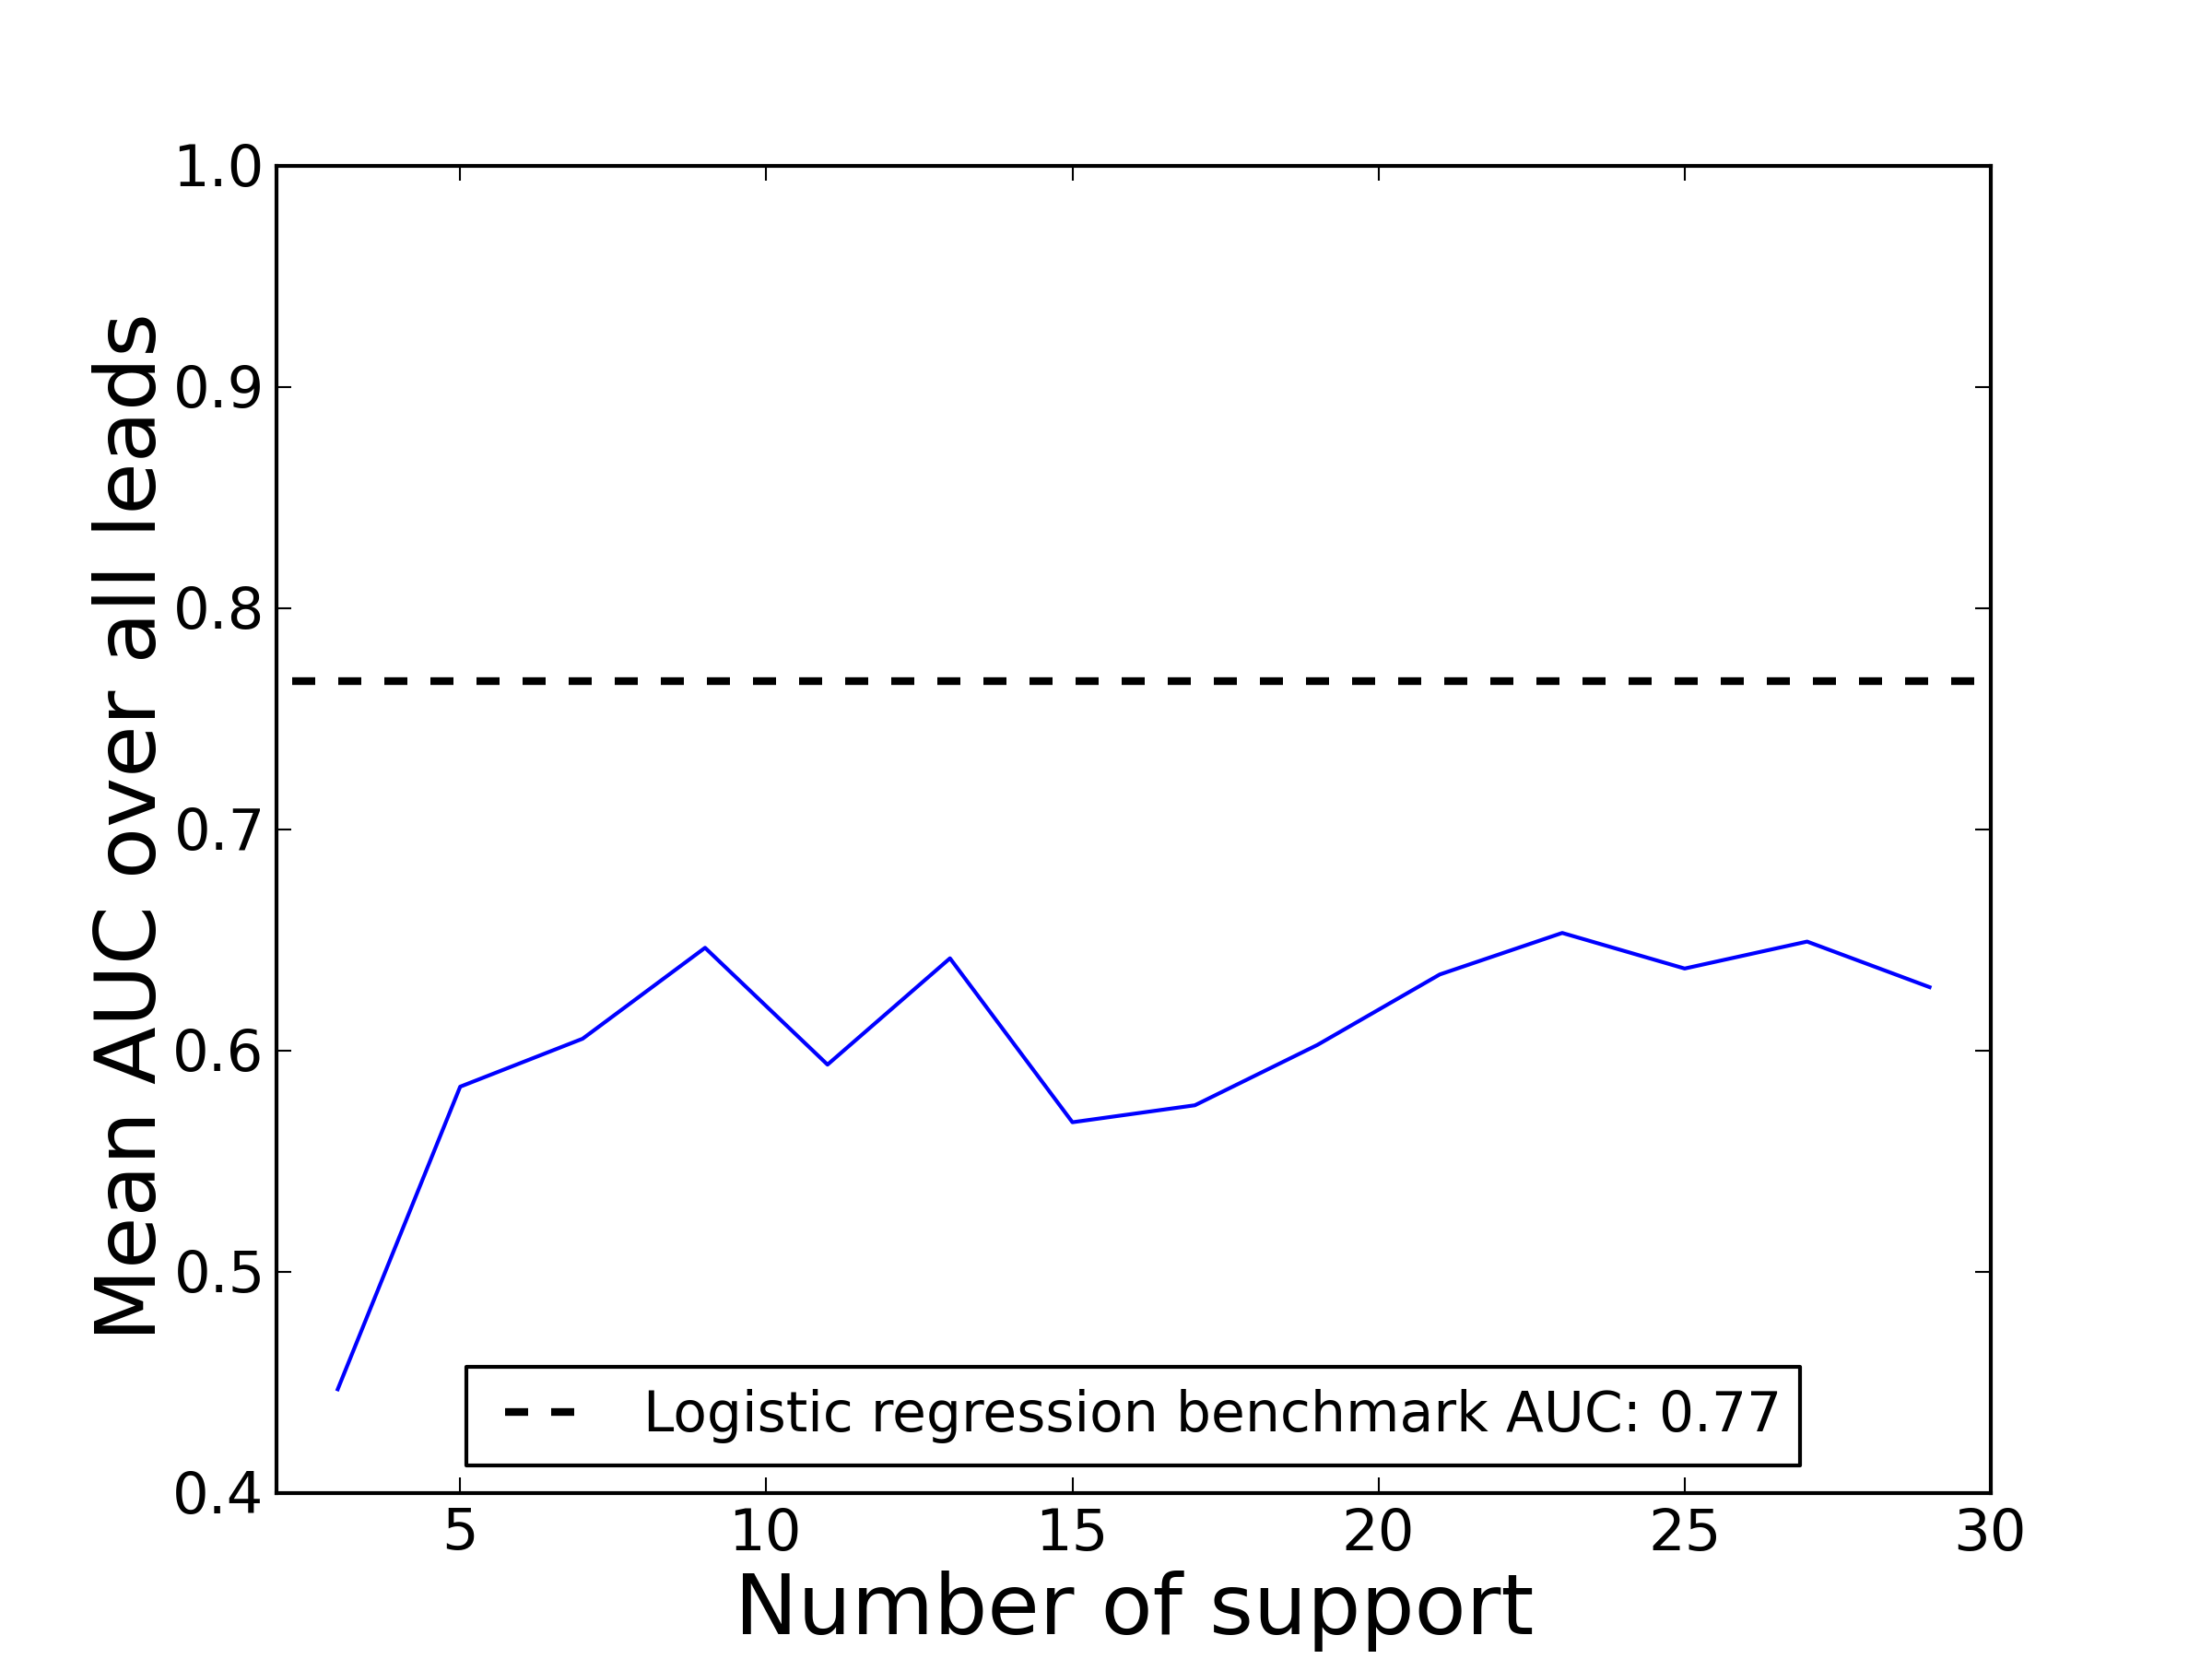
\includegraphics[width=0.8\textwidth]{figures/hmm/forum_only_pca_support_over_time.png}
\end{figure}

\begin{figure}[ht!]
  \caption{Mean AUC as K increases for the \both cohort. PCA transformations of features used.}\label{fig:hmm_support_over_time_forum_and_wiki_pca}
  \centering
    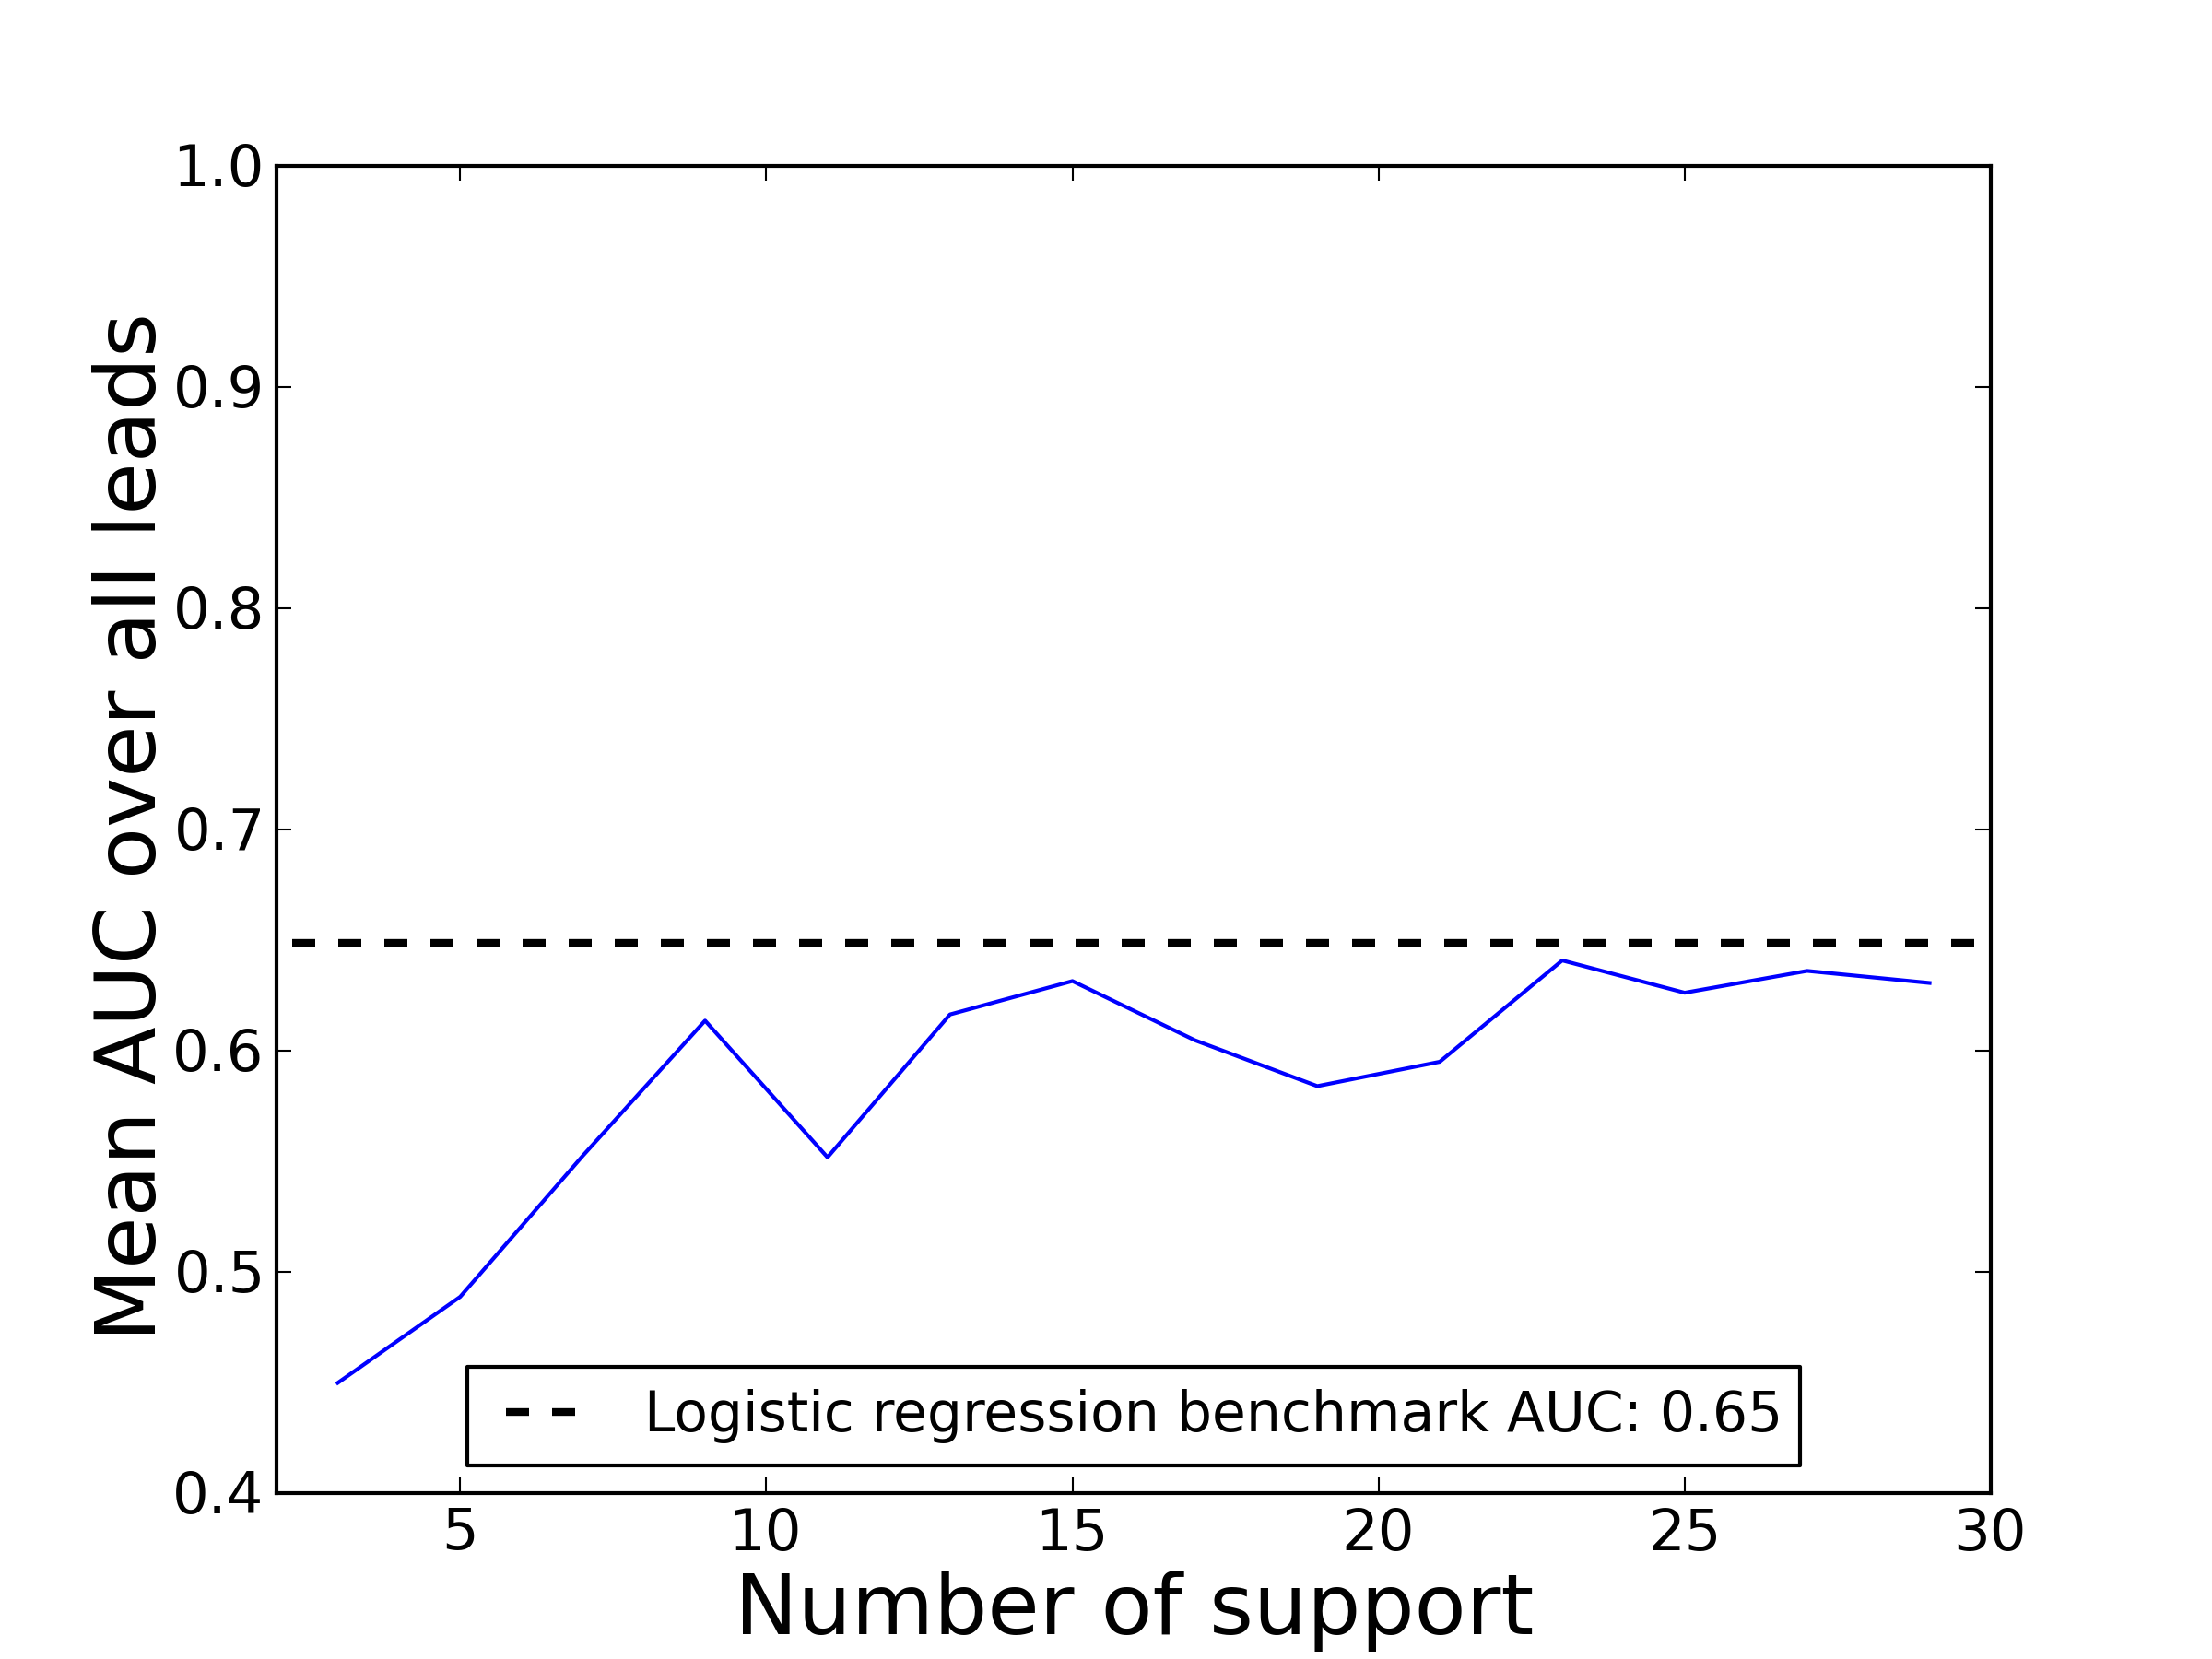
\includegraphics[width=0.8\textwidth]{figures/hmm/forum_and_wiki_pca_support_over_time.png}
\end{figure}


The following line graphs show how overall predictive accuracies of the PCA HMM models change as K increases. These graphs indicate the correct number of hidden states needed in order to model each cohort. See Figures \ref{fig:hmm_support_over_time_no_collab_pca} through 
\ref{fig:hmm_support_over_time_forum_and_wiki_pca}. The mean prediction AUC of all 91 experiments for logistic regression is also shown for each cohort as a benchmark.

The results again indicate that the \forum and \both cohorts seem to have converged, but not until K has reached ~25. However, the \neither cohort's mean AUC is still increasing as K goes to 29, indicating that a higher K could better model this cohort.

\begin{figure}[ht!]
  \caption{Heatmap for the \neither cohort.}\label{fig:hmm_heatmap_no_collab}
  \centering
    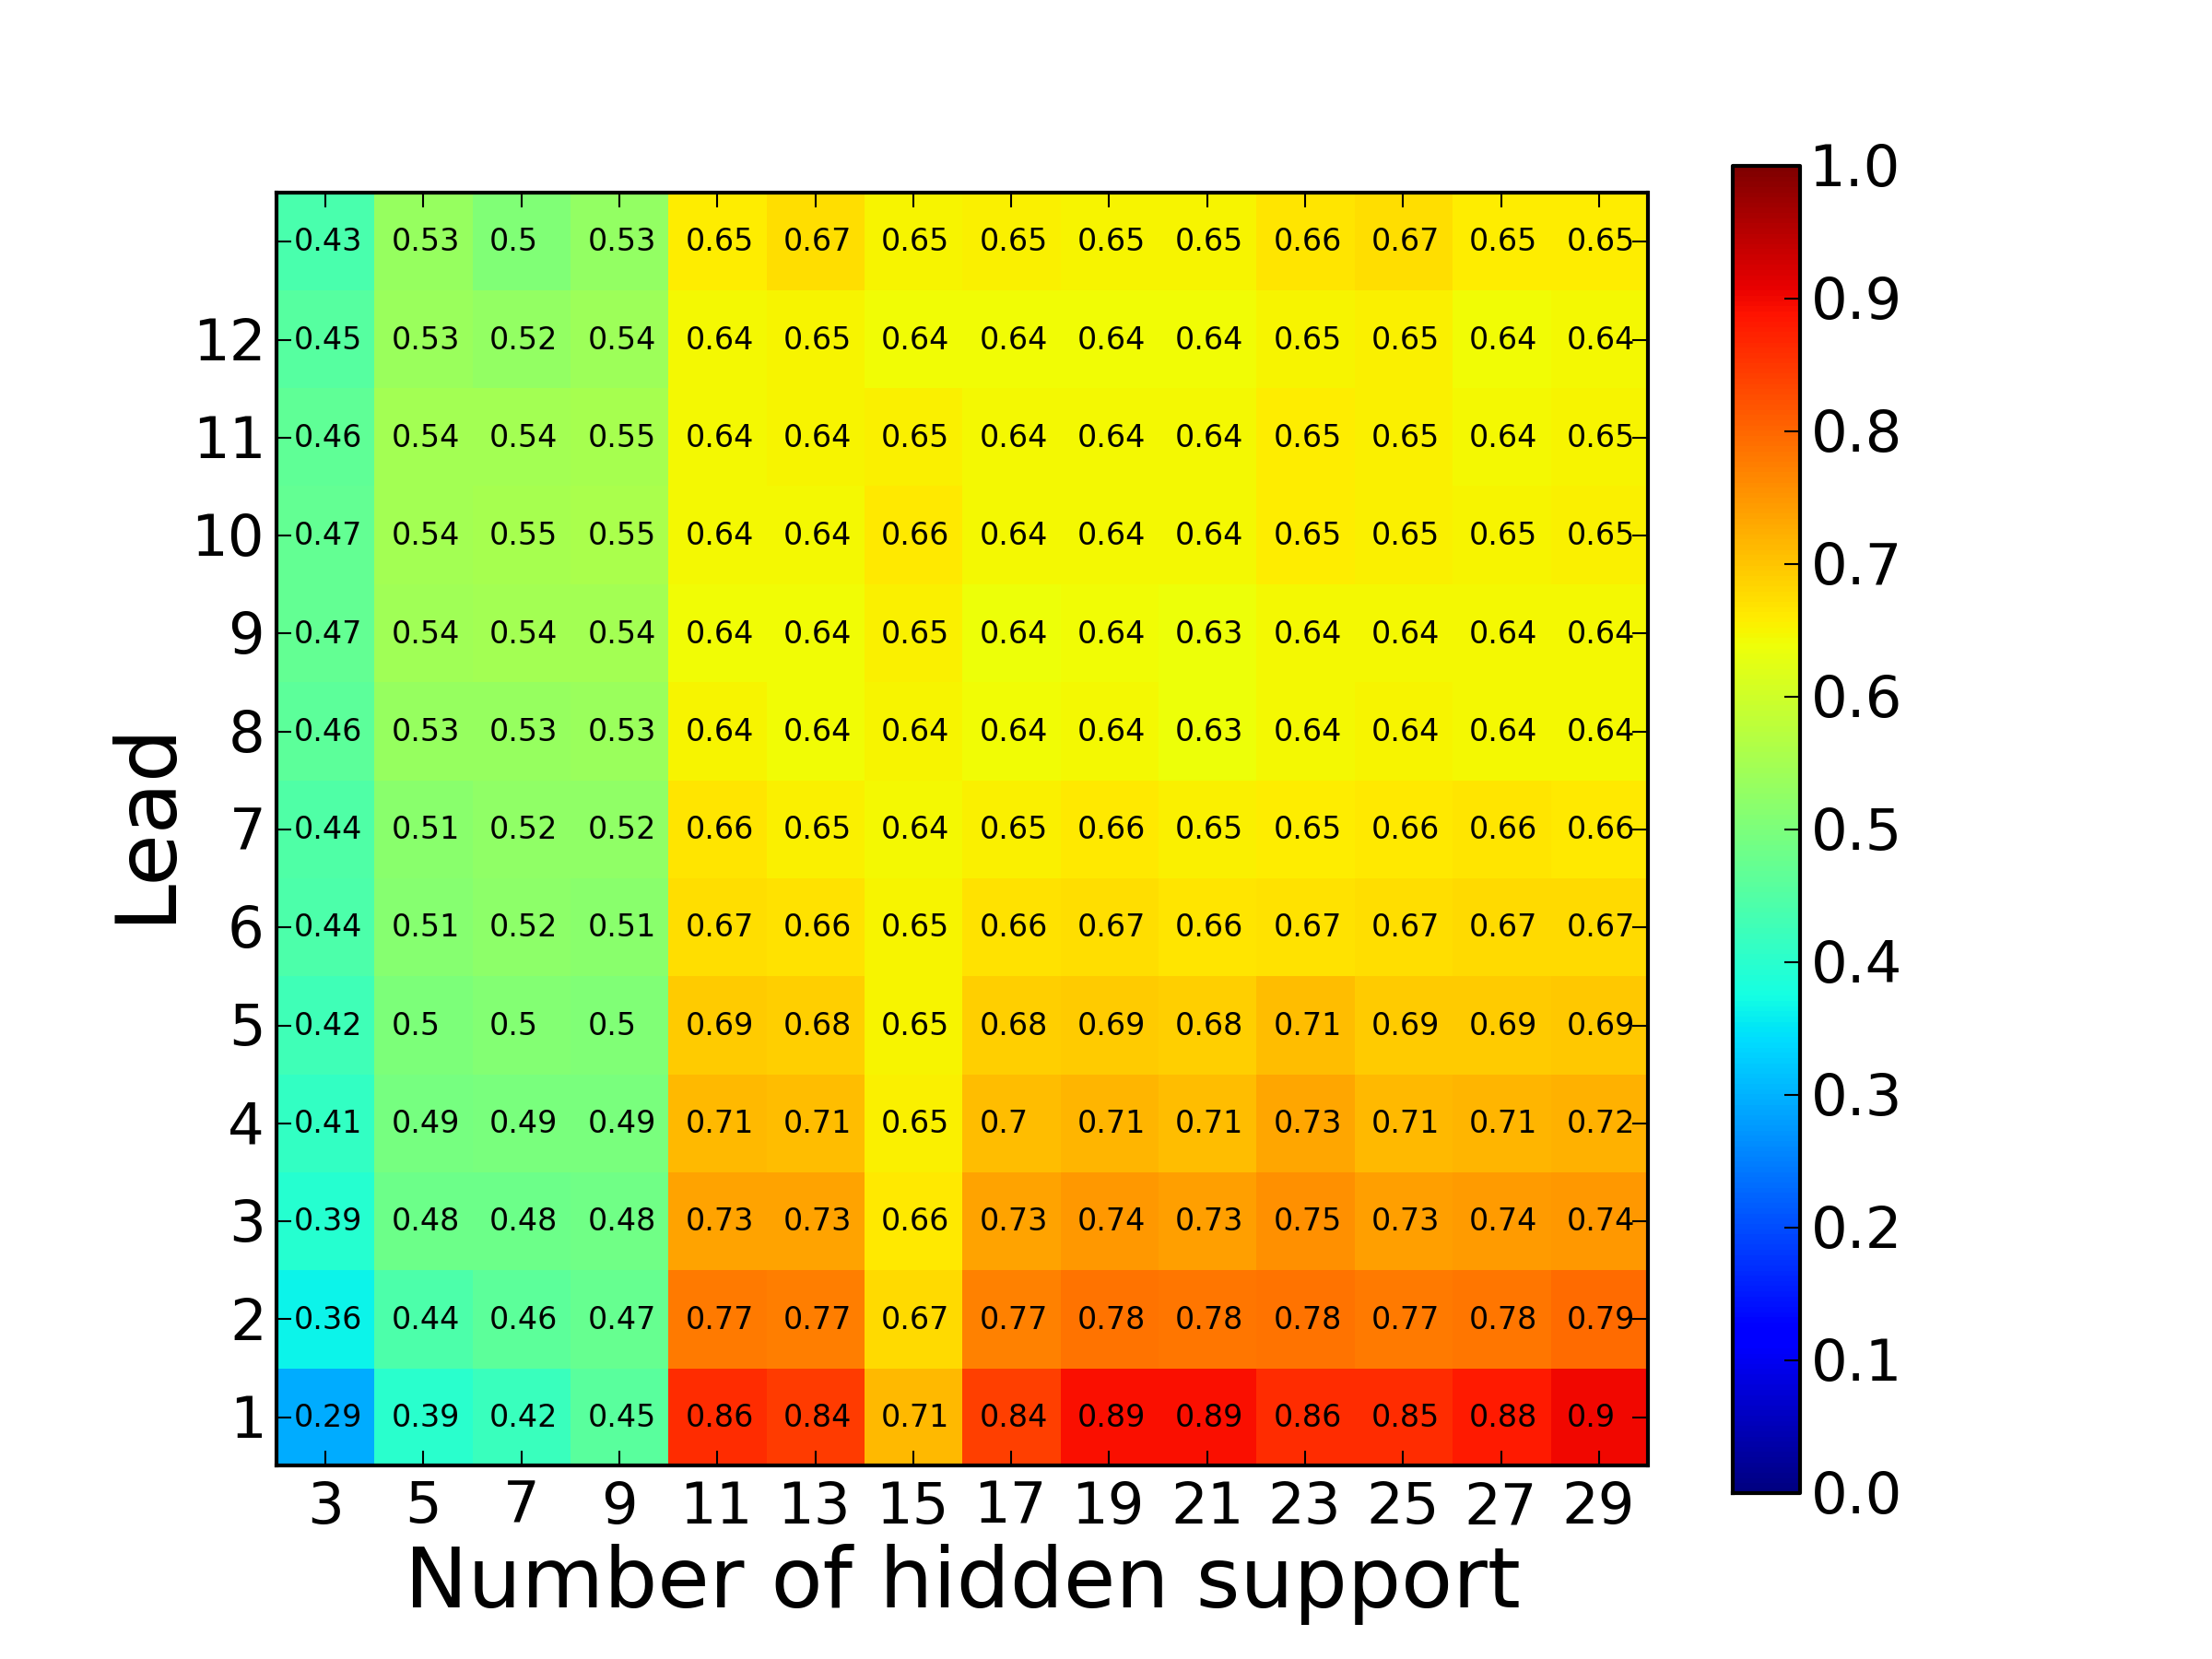
\includegraphics[width=1.0\textwidth]{figures/hmm/no_collab.png}
\end{figure}

\begin{figure}[ht!]
  \caption{Heatmap for the \forum cohort.}\label{fig:hmm_heatmap_forum_only}
  \centering
    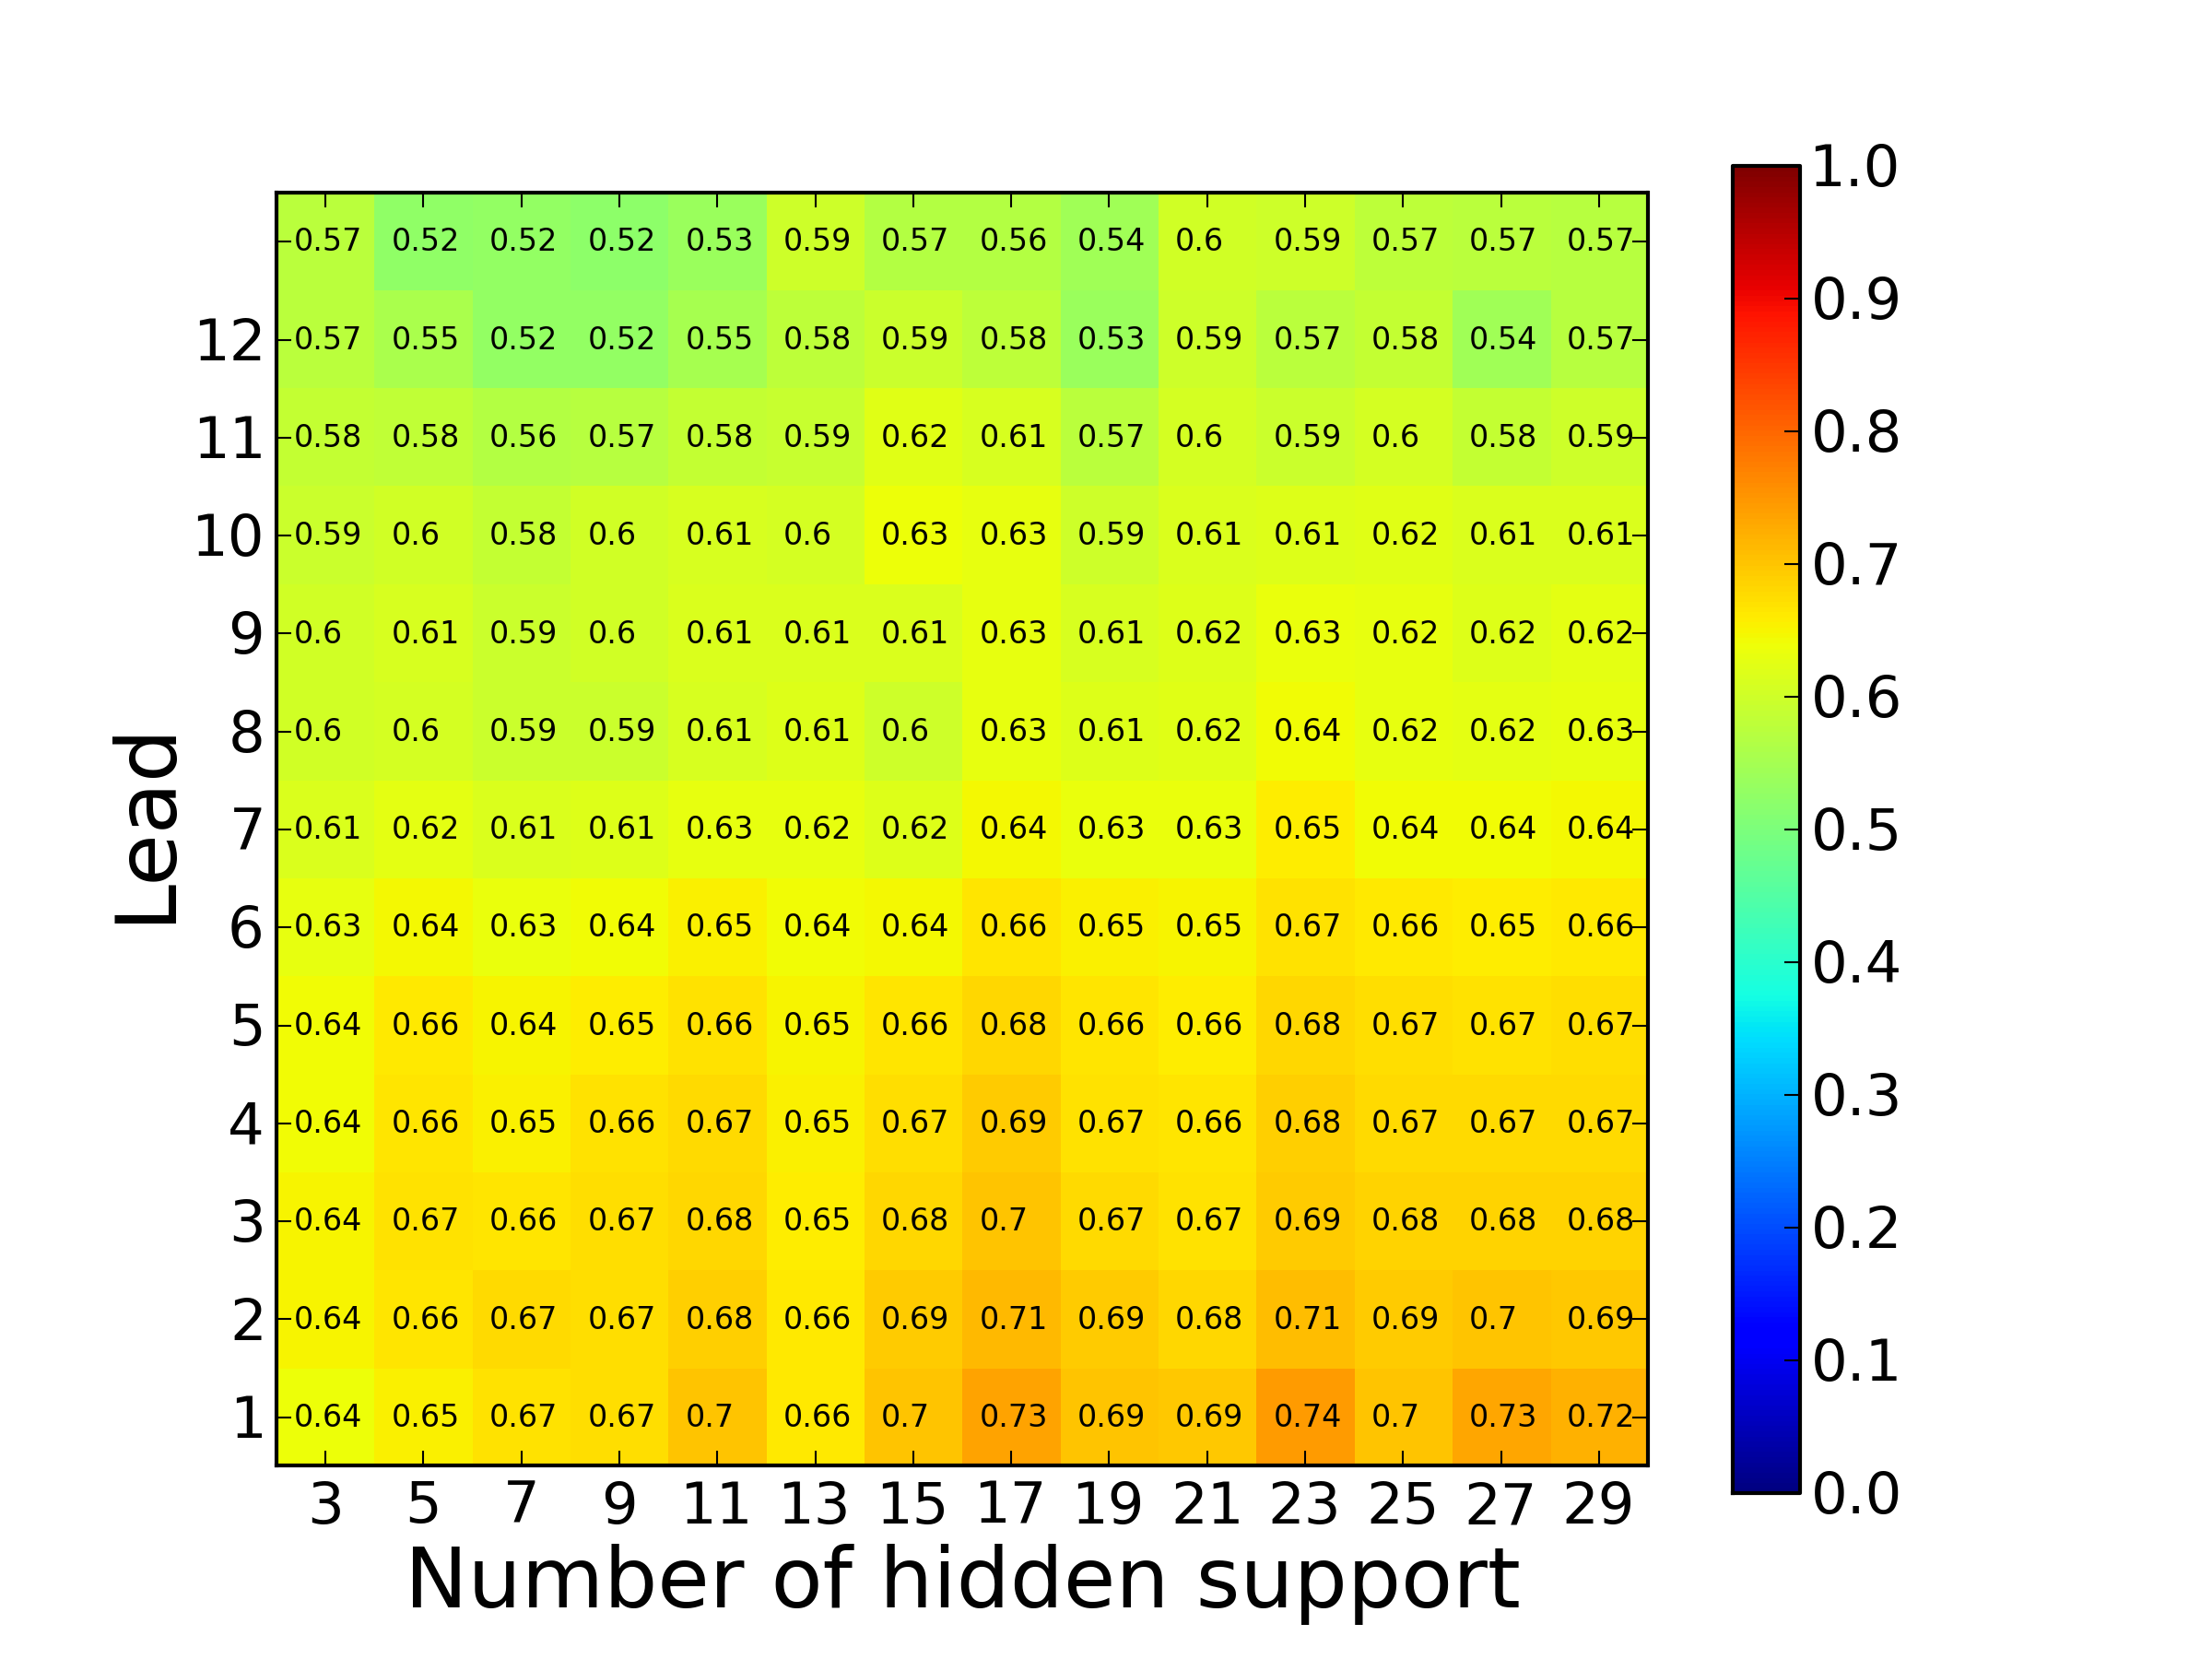
\includegraphics[width=1.0\textwidth]{figures/hmm/forum_only.png}
\end{figure}

\begin{figure}[ht!]
  \caption{Heatmap for the \both cohort.}\label{fig:hmm_heatmap_forum_and_wiki}
  \centering
    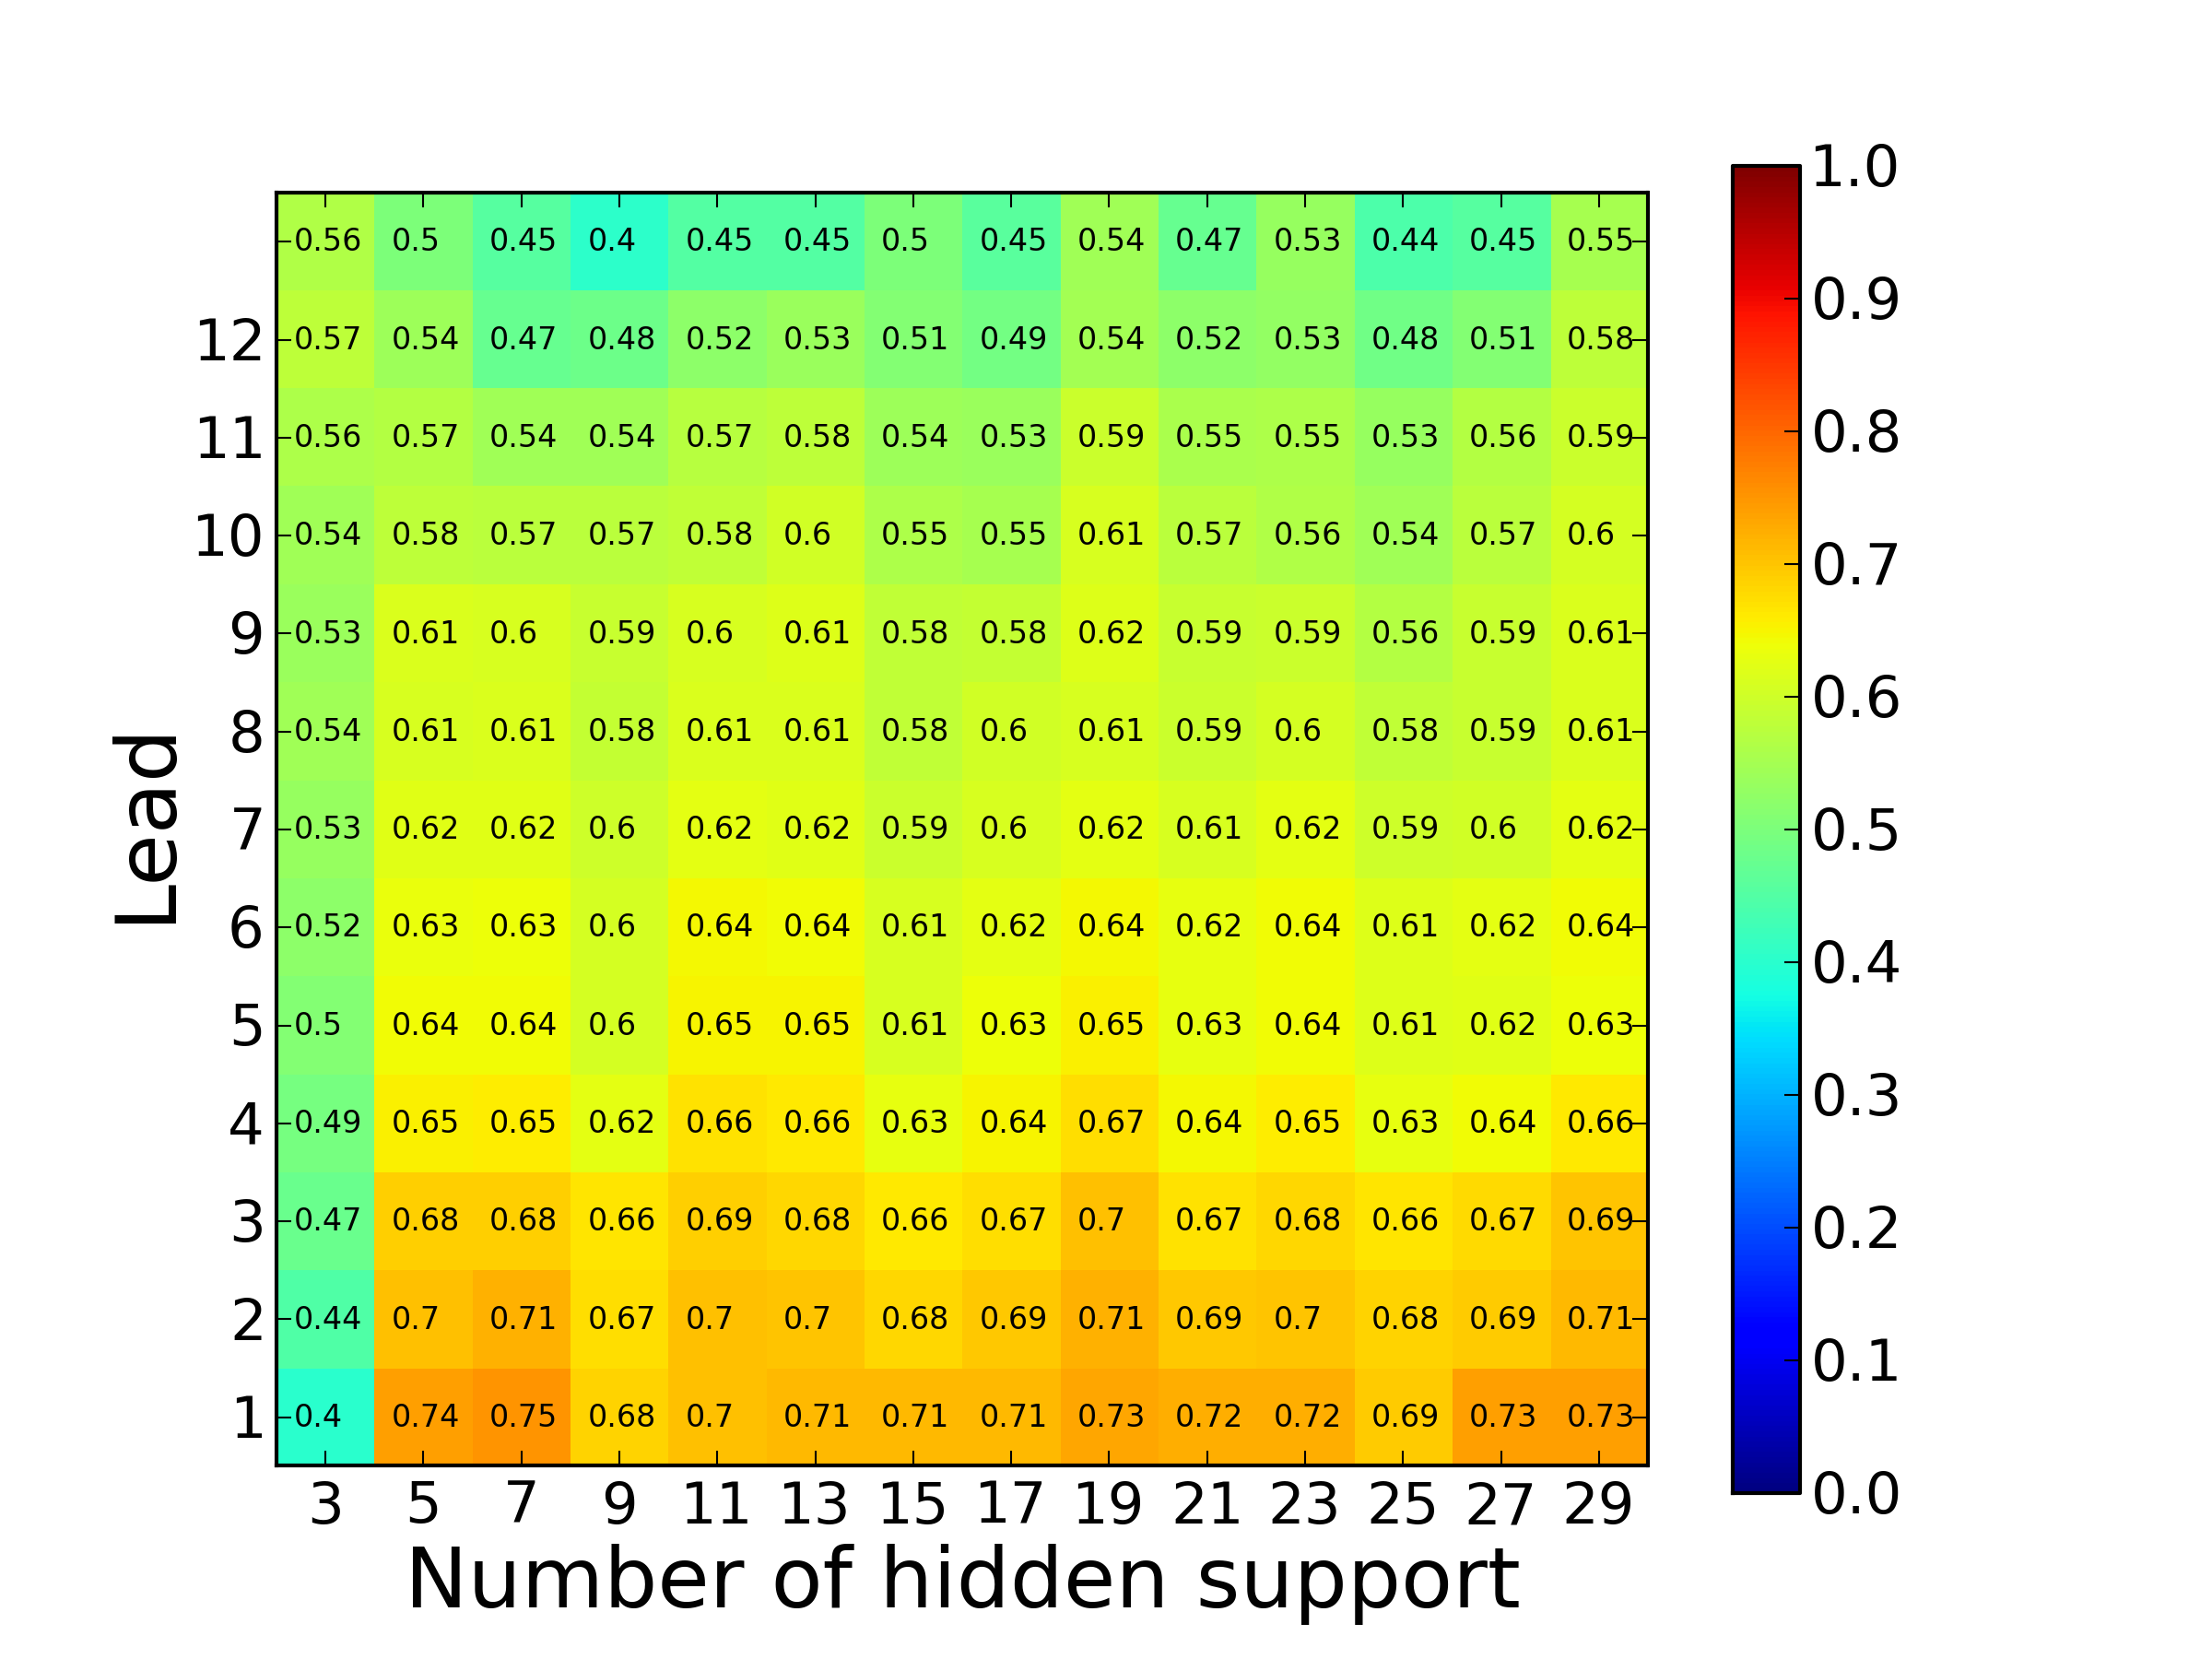
\includegraphics[width=1.0\textwidth]{figures/hmm/forum_and_wiki.png}
\end{figure}

\begin{figure}[ht!]
  \caption{Heatmap for the \wiki cohort.}\label{fig:hmm_heatmap_wiki_only}
  \centering
    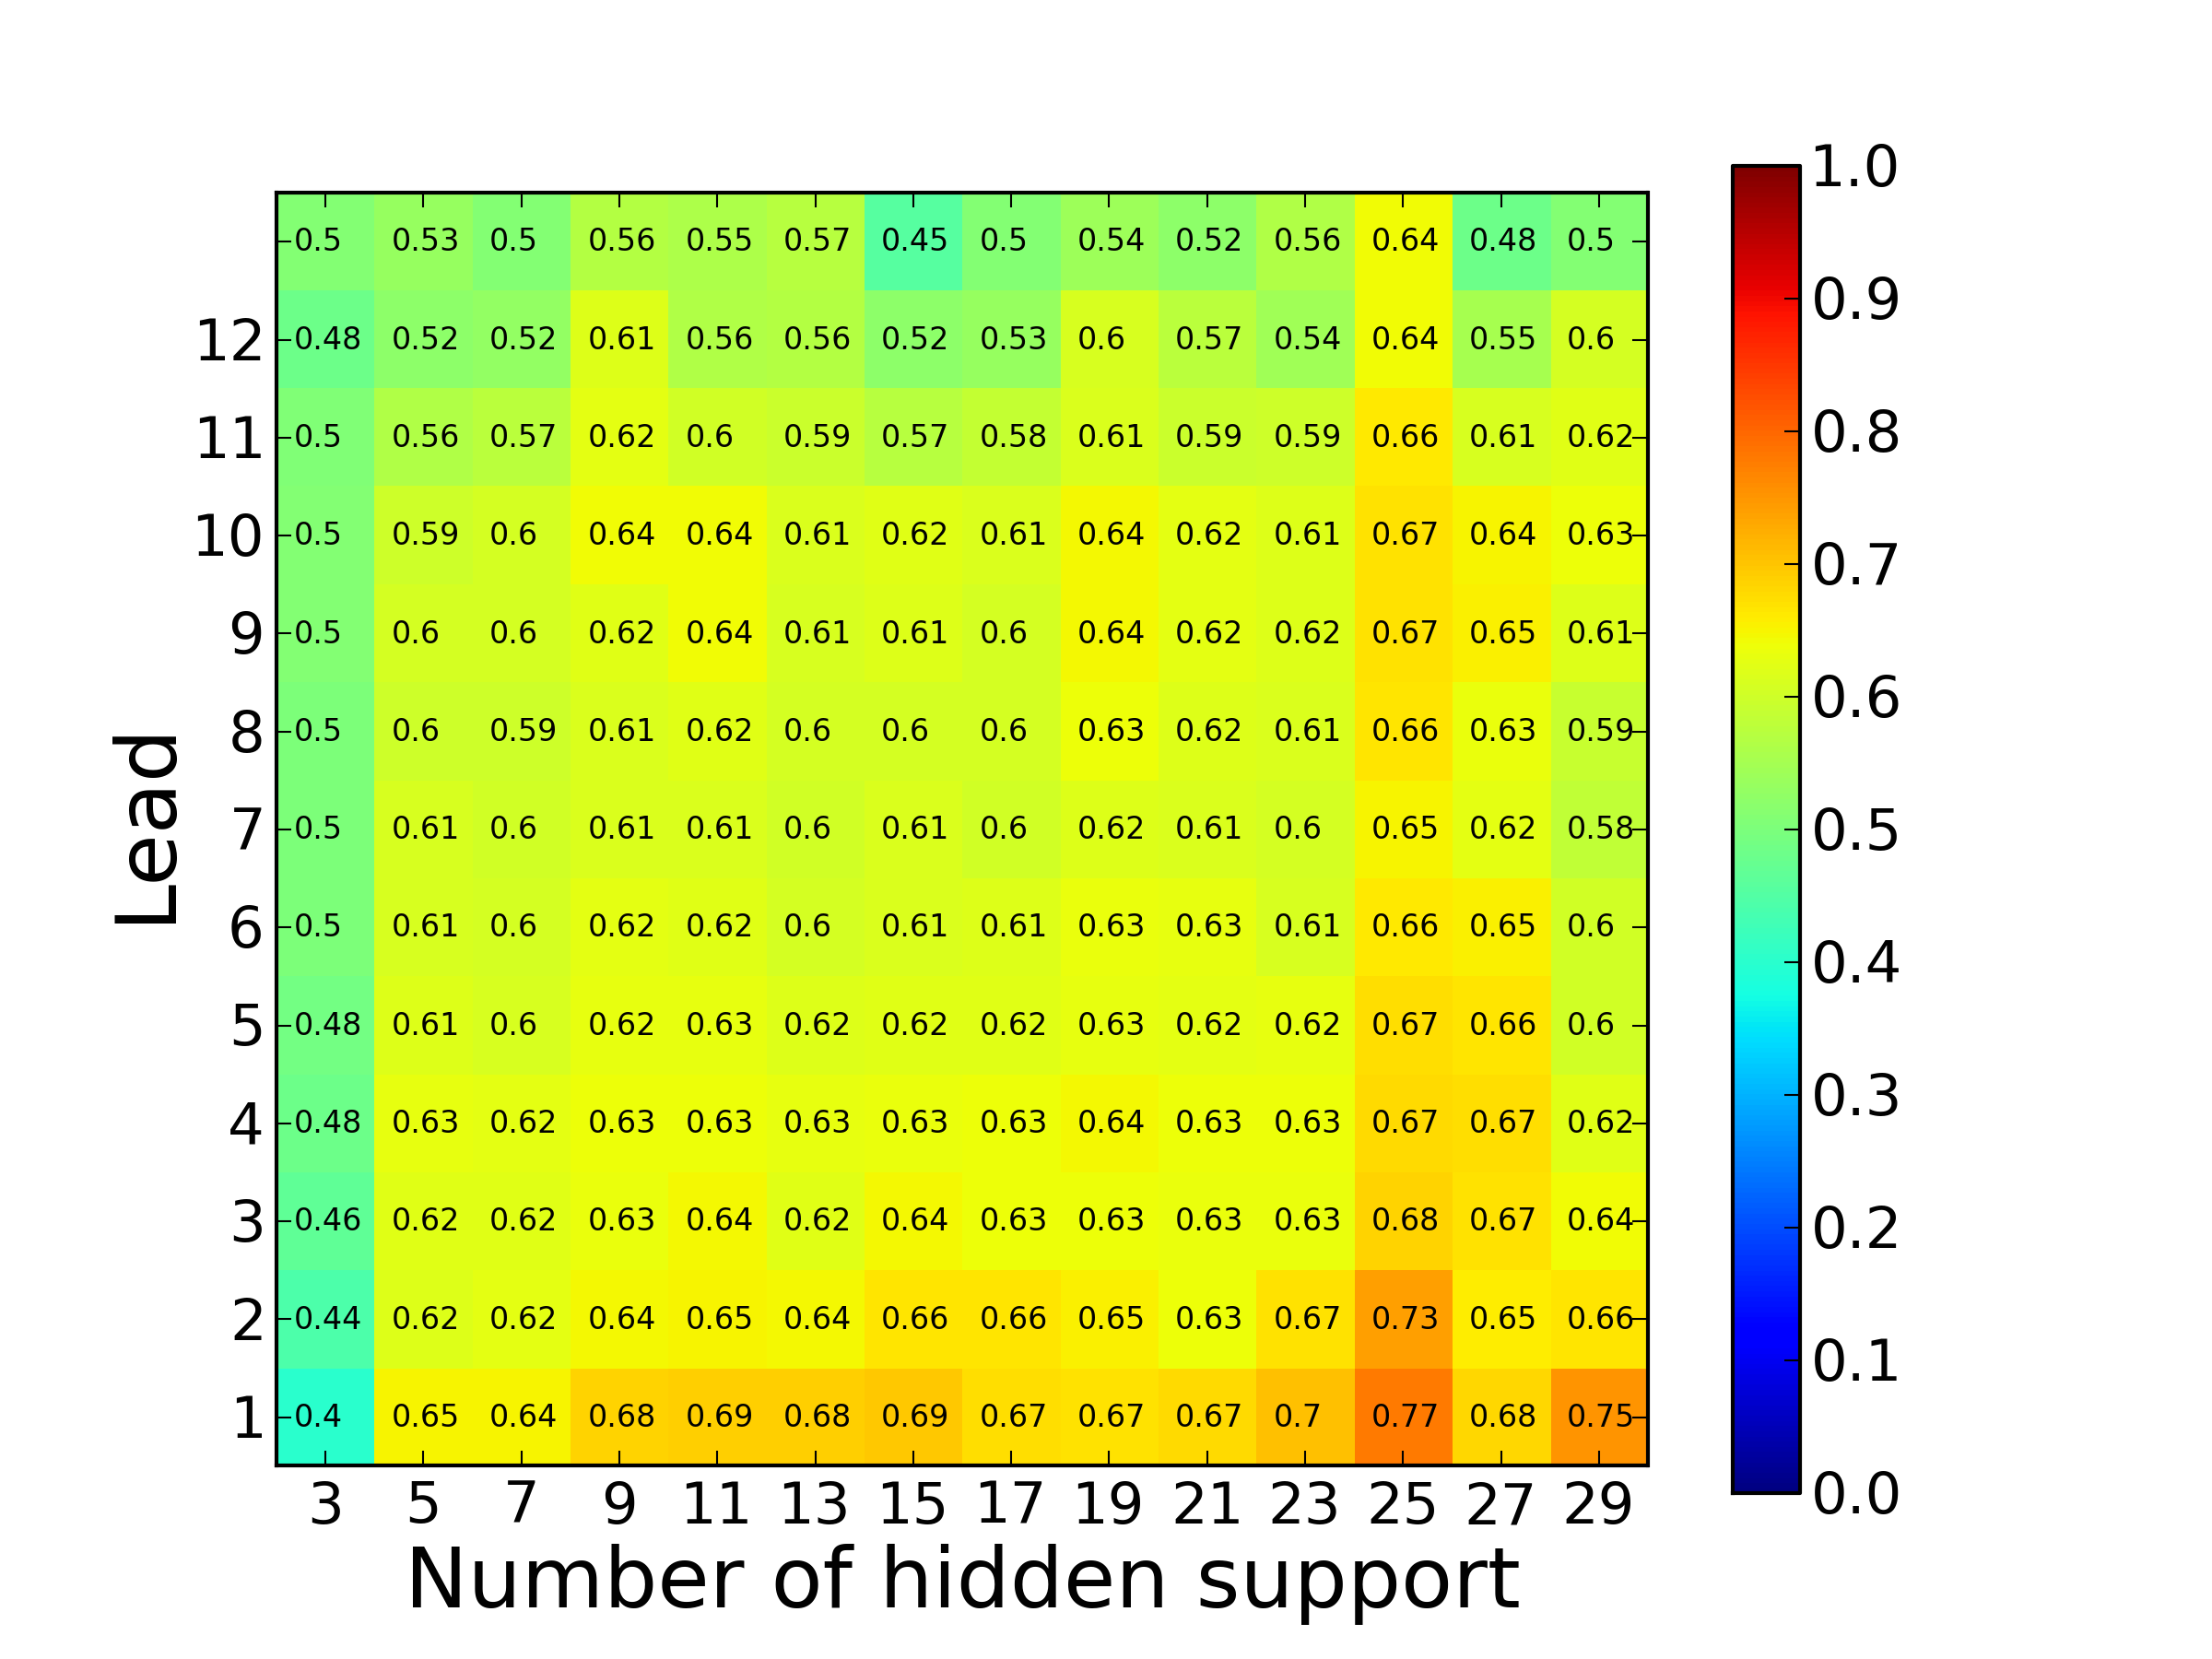
\includegraphics[width=1.0\textwidth]{figures/hmm/wiki_only.png}
\end{figure}

Figures \ref{fig:hmm_heatmap_no_collab} to \ref{fig:hmm_heatmap_wiki_only} show HMM heatmaps for all four cohorts using features that did not undergo principal component analysis. Interestingly, they achieved much different results than the HMMs with PCA. For example, Figure \ref{fig:hmm_heatmap_no_collab} performs consistently better than its PCA counterpart. It converges more quickly- achieving near optimal predictive power at K = 11. It outperforms PCA in nearly every experiment (given K greater than 9), and even attains an AUC of 0.9. This provides further evidence that the PCA HMM did not converge, and it could achieve results as good with a higher K.

However, for other cohorts, such as \forum, the PCA HMM \ref{fig:hmm_heatmap_forum_only} consistently out-predicts the HMM without PCA. The PCA HMM achieves an AUC of ~.78 for all K greater than 19 and lead of one, whereas its non-PCA HMM only hits ~0.82. Similar differences exist in the \both cohort in \ref{fig:hmm_heatmap_forum_and_wiki}. In both of these cohorts, it appears that the PCA HMM used a high enough K to converge to the correct number of modes of students.

One last difference between the non-PCA HMMs and the PCA HMMs is that the non-PCA model's predictive power degrades more gracefully as the lead increases. This remains to be explained and requires more investigation.

\begin{figure}[ht!]
  \caption{Mean AUC as K increases for the \neither cohort.}\label{fig:hmm_support_over_time_no_collab}
  \centering
    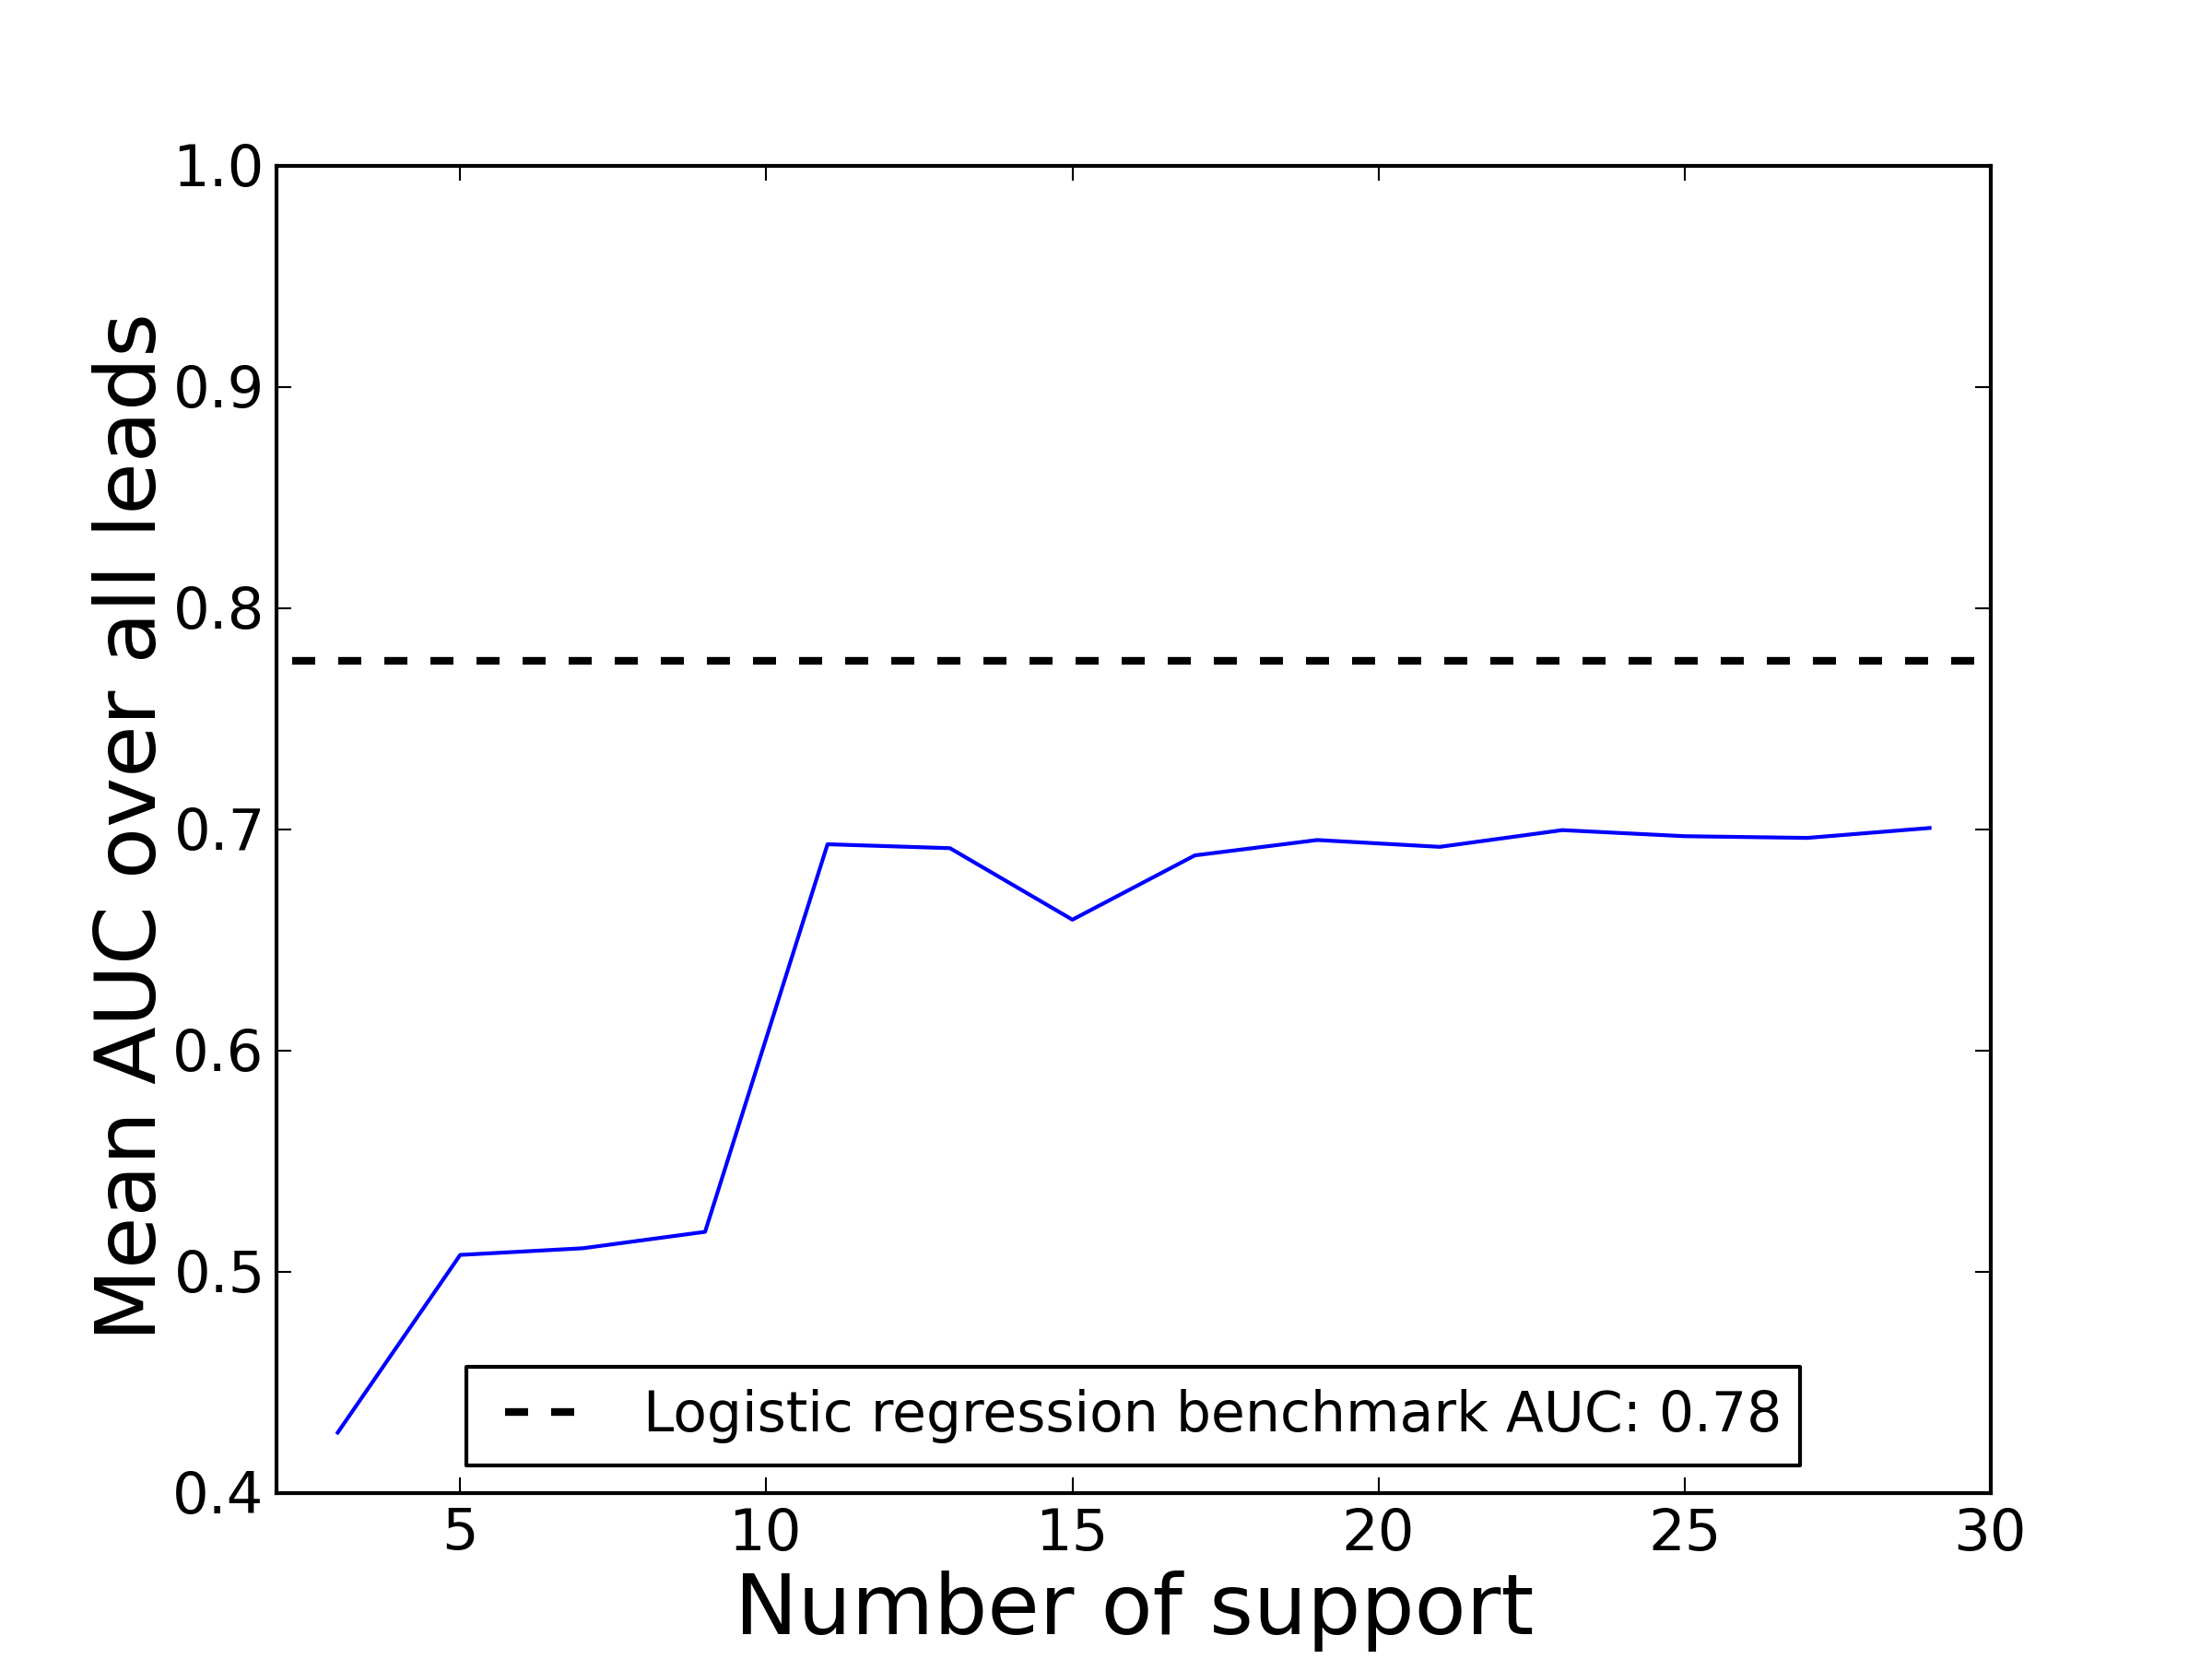
\includegraphics[width=0.8\textwidth]{figures/hmm/no_collab_support_over_time.png}
\end{figure}

\begin{figure}[ht!]
  \caption{Mean AUC as K increases for the \forum cohort.}\label{fig:hmm_support_over_time_forum_only}
  \centering
    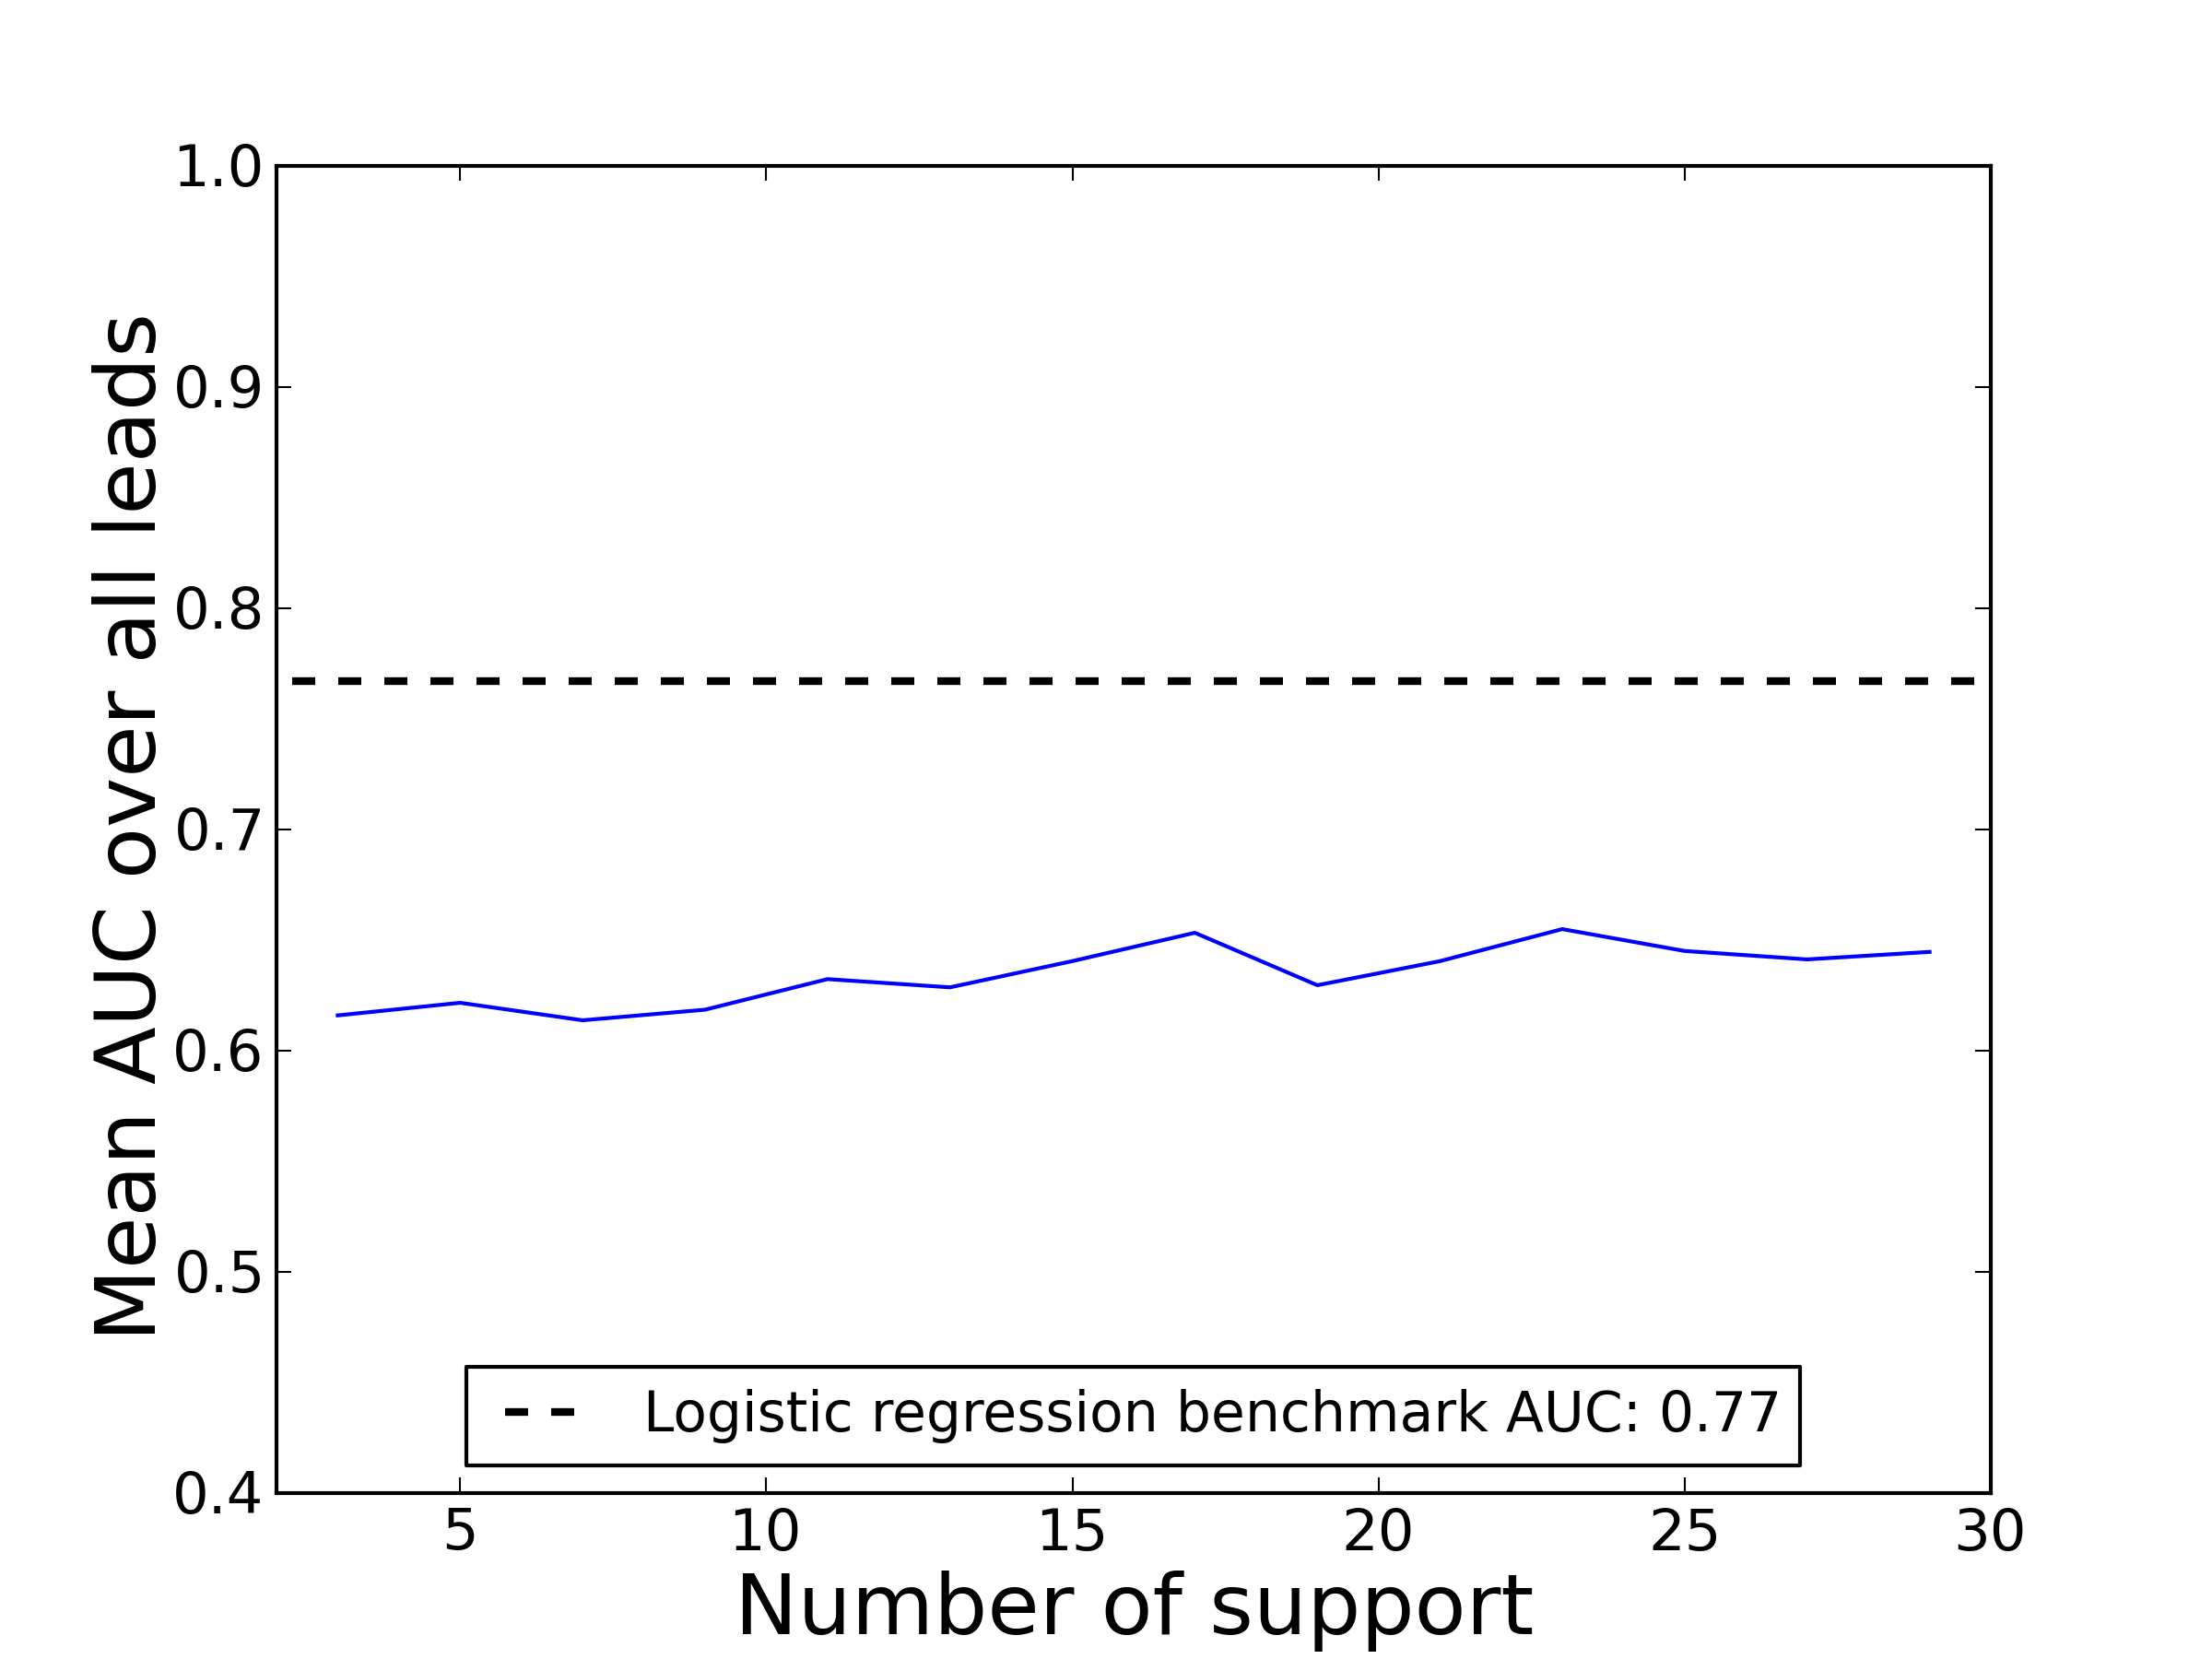
\includegraphics[width=0.8\textwidth]{figures/hmm/forum_only_support_over_time.png}
\end{figure}

\begin{figure}[ht!]
  \caption{Mean AUC as K increases for the \both cohort.}\label{fig:hmm_support_over_time_forum_and_wiki}
  \centering
    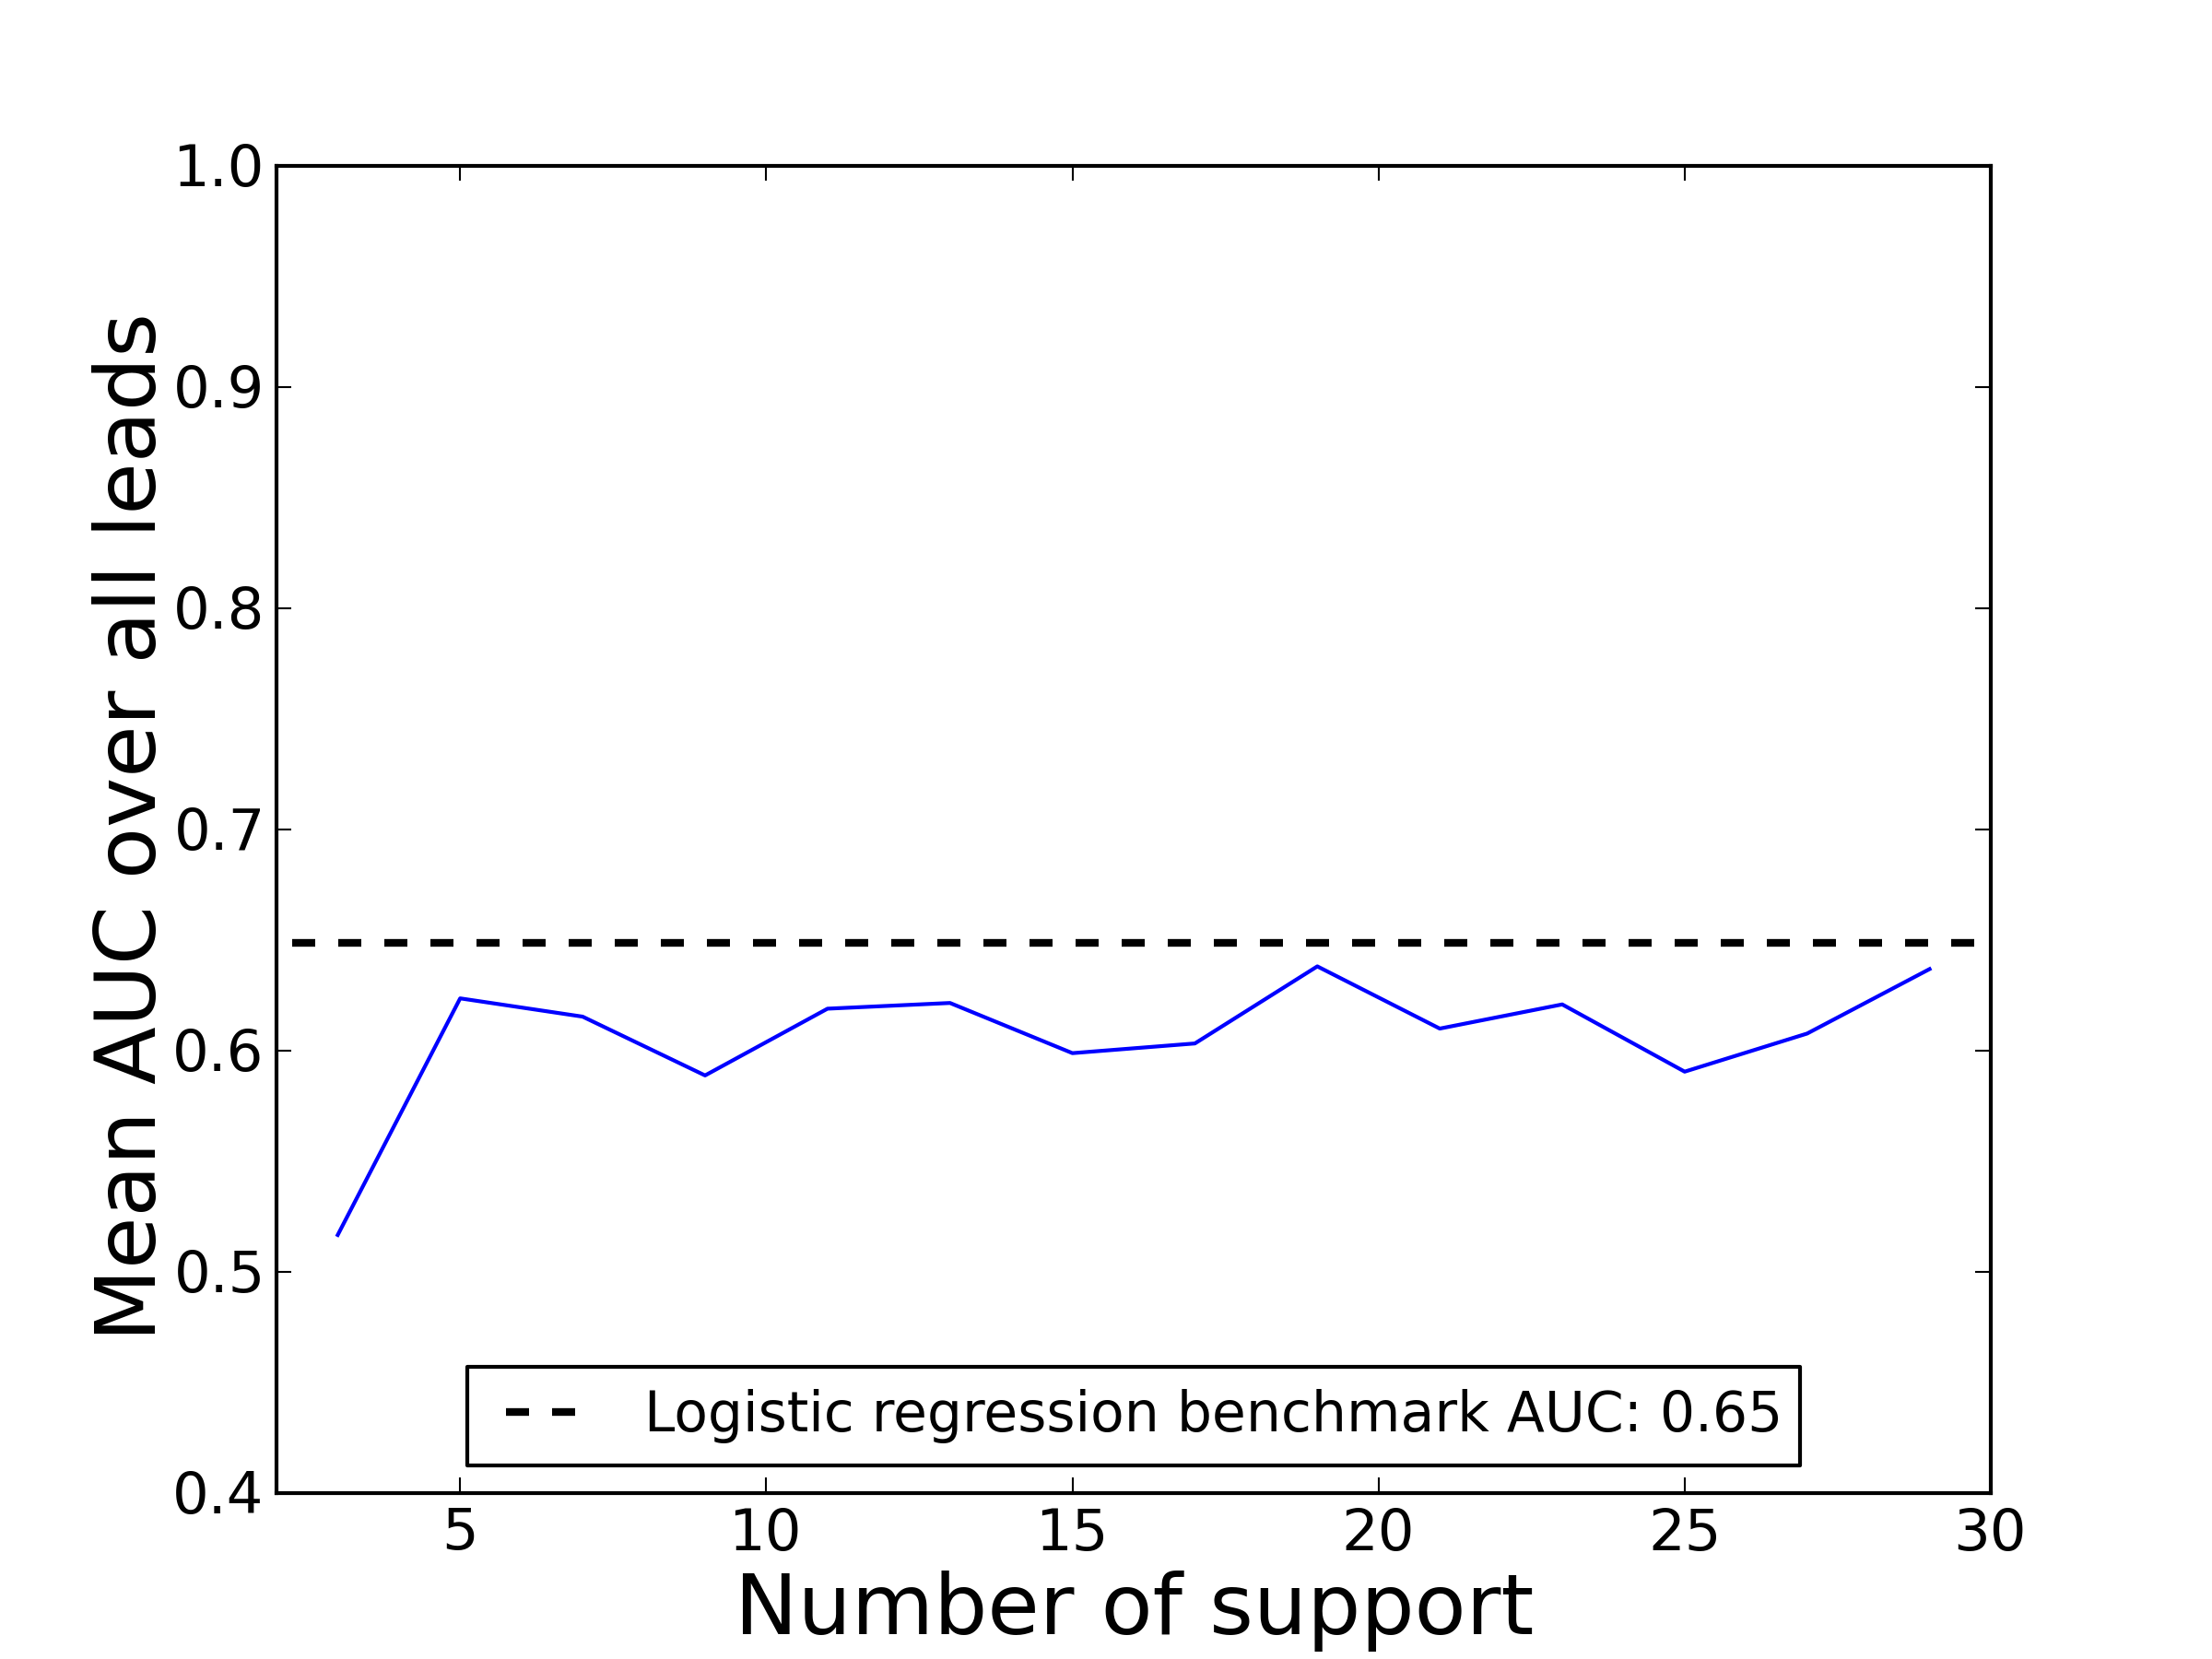
\includegraphics[width=0.8\textwidth]{figures/hmm/forum_and_wiki_support_over_time.png}
\end{figure}

\begin{figure}[ht!]
  \caption{Mean AUC as K increases for the \wiki cohort.}\label{fig:hmm_support_over_time_wiki_only}
  \centering
    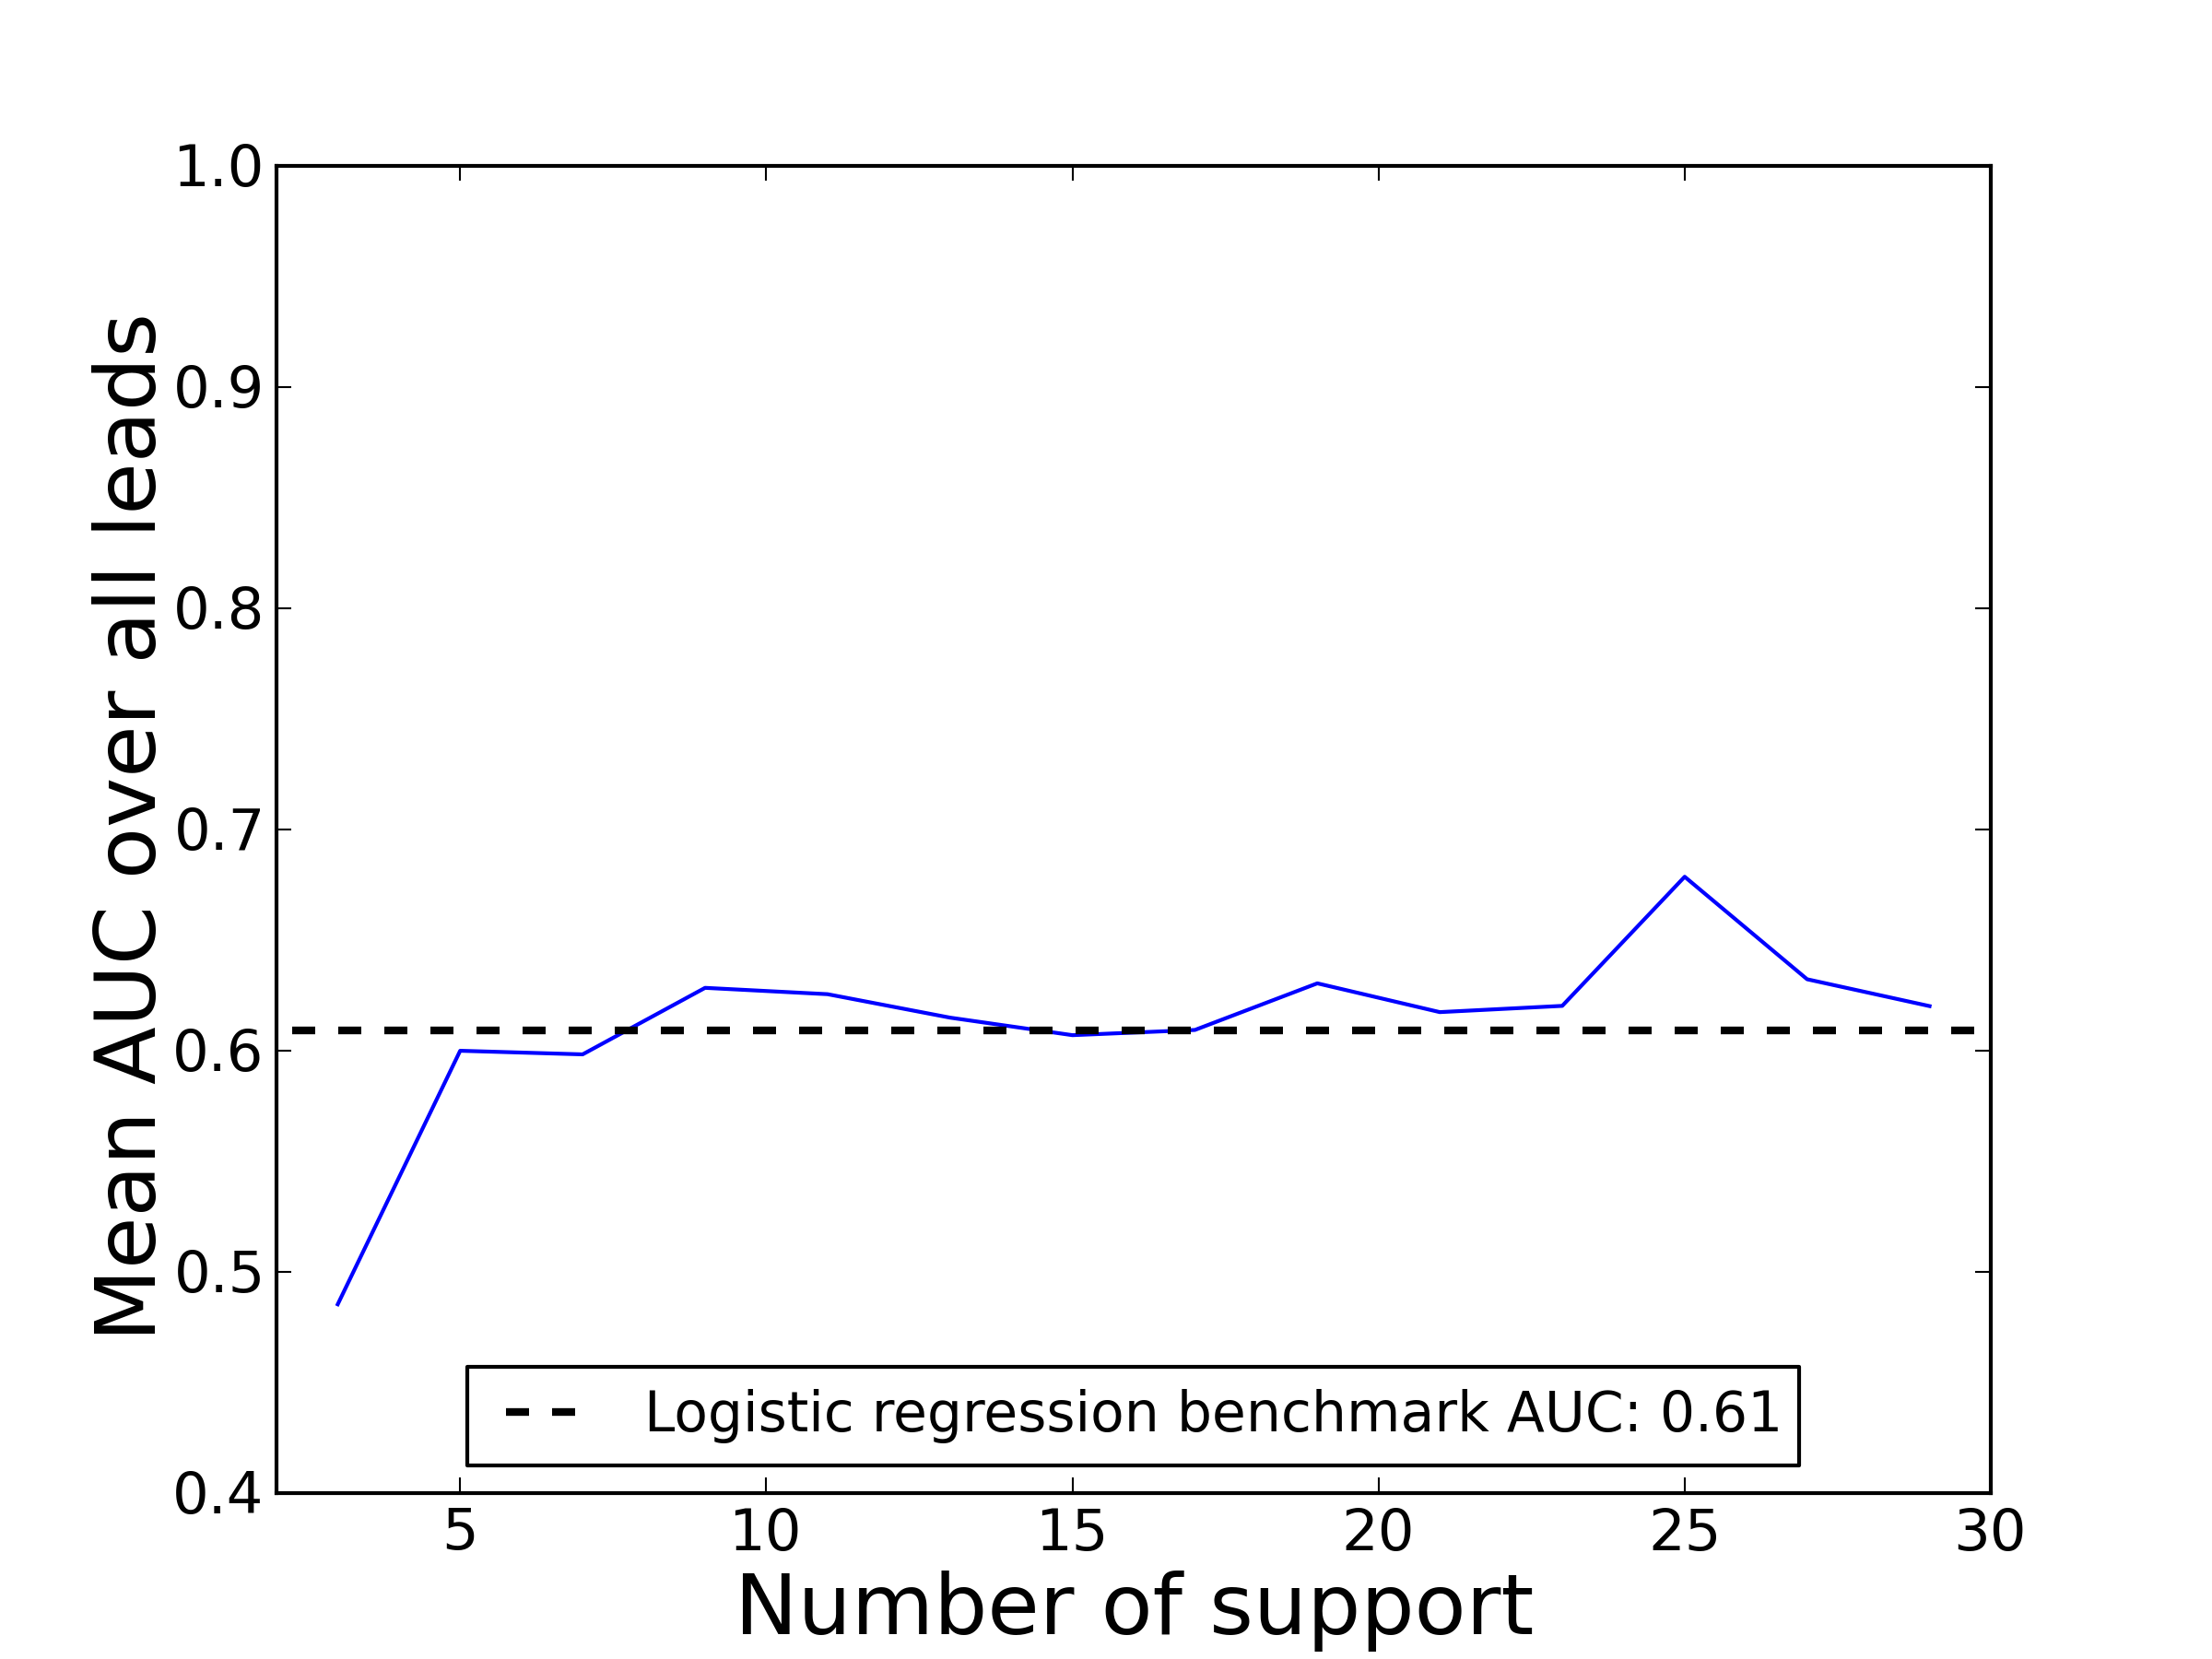
\includegraphics[width=0.8\textwidth]{figures/hmm/wiki_only_support_over_time.png}
\end{figure}

In figures \ref{fig:hmm_support_over_time_no_collab} through \ref{fig:hmm_support_over_time_wiki_only} we look at how the mean AUC changes as K increases for the non-PCA HMMs. We see the AUCs converge much faster than the PCA HMMs. In addition, the mean AUC comes closer to the benchmark logistic regression mean AUC. This is especially true for the smaller \wiki and \both cohorts, on which logistic regression performs poorly due to a lack of data. Indeed, the \wiki HMM outperforms its logistic regression counterpart for almost all values of K.

At this point in the thesis, Chapter \ref{chap:logreg} has described models with logistic regression and Chapter \ref{chap:hmm} with HMMs. HMMs rarely generated AUC results better than logistic regression and were more predictively accurate when we used features not reduced by PCA. Perhaps the best value derived from HMMs is the insight into a hidden state and its support. In Chapter \ref{chap:logreg_hmm} attempt to leverage the hidden state unmasked by HMMs can be used with logistic regression modelling to further extend prediction.







% \begin {center}
% \begin {tikzpicture}[-latex ,auto ,node distance =4 cm and 5cm ,on grid ,
% semithick ,
% state/.style ={ circle ,top color =white , bottom color = processblue!20 ,
% draw,processblue , text=blue , minimum width =1 cm}]
% \node[state] (C)
% {$1$};
% \node[state] (A) [above left=of C] {$0$};
% \node[state] (B) [above right =of C] {$2$};
% \path (A) edge [loop left] node[left] {$1/4$} (A);
% \path (C) edge [bend left =25] node[below =0.15 cm] {$1/2$} (A);
% \path (A) edge [bend right = -15] node[below =0.15 cm] {$1/2$} (C);
% \path (A) edge [bend left =25] node[above] {$1/4$} (B);
% \path (B) edge [bend left =15] node[below =0.15 cm] {$1/2$} (A);
% \path (C) edge [bend left =15] node[below =0.15 cm] {$1/2$} (B);
% \path (B) edge [bend right = -25] node[below =0.15 cm] {$1/2$} (C);
% \end{tikzpicture}
% \end{center}